\documentclass[11pt]{article}
\usepackage[utf8]{inputenc}
\usepackage[english]{babel}
\usepackage{amsmath}
\usepackage{graphicx}
\usepackage{float}
\usepackage{lipsum}
\usepackage{multicol}
\usepackage{xcolor}
\usepackage{tabularx}
\usepackage{booktabs}
\usepackage{subfigure}
\usepackage{hyperref}
\usepackage{listings}
\newcolumntype{Y}{>{\centering\arraybackslash}X}
\usepackage[left=2.00cm, right=2.00cm, top=2.00cm, bottom=2.00cm]{geometry}

\title{IACV project report}

\begin{document}

\begin{figure}[H]
    \centering
    
\includegraphics[scale=0.4]{polimi.png}
    % \includegraphics[scale=0.175]{edison.png} \hfill \includegraphics[scale=0.3]{airlab.jpeg}
\end{figure}

% \vspace{5mm}

\begin{center}
    % Select between First and Second
    {\Large \textbf{Image Analysis and Computer Vision}}\\
    \vspace{2mm}
    % Change with your Team Name
    {\Large \textbf{Project report}}\\
    \vspace{2mm}
    % Team Members Information

    {\large Elia Pontiggia}\\
    \vspace{2mm}
    % Codabench Nicknames
    {247274 - 10716792}\\

    \vspace{5mm}
    {\Large \textbf{Proposal F02: Reconstructing drone trajectories and cameras from multiple images}}\\
    \vspace{3mm}
    \today
\end{center}
\vspace{5mm}

\begin{figure}[H]
    \centering
    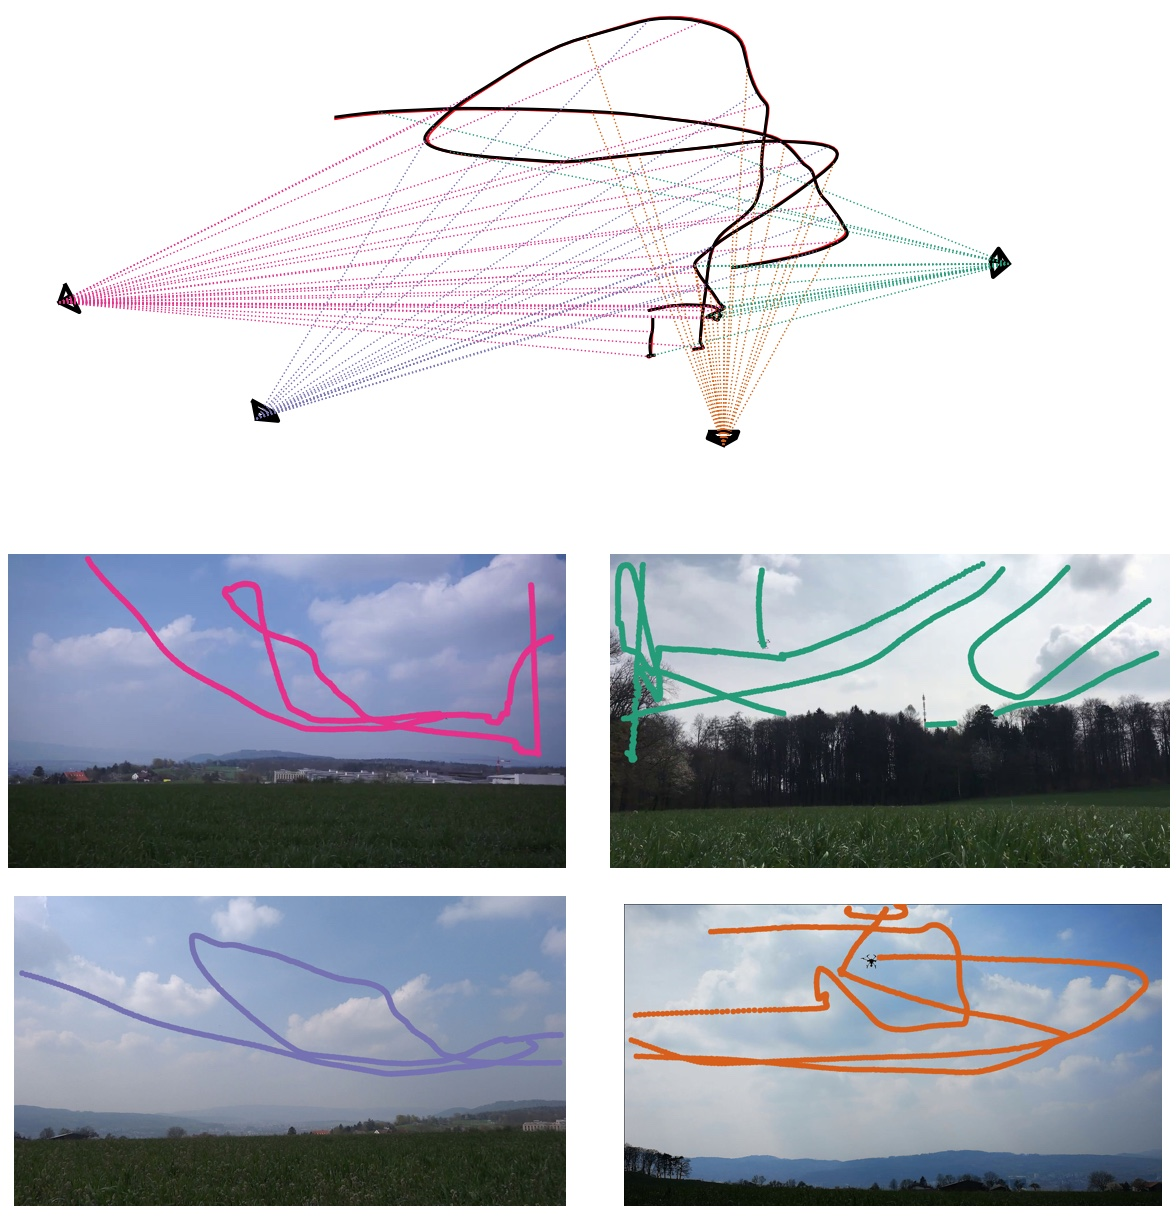
\includegraphics[width=0.75\textwidth]{imgs/cover.jpg}
\end{figure}

\tableofcontents

\section{Introduction}

\subsection{Problem Formulation}
With the growing ubiquity of unmanned aerial vehicles (UAVs) across industries—ranging from cinematography to environmental monitoring—accurately tracking their motion in three-dimensional space has become increasingly vital. While onboard navigation systems using GNSS, IMUs, or visual-inertial odometry are widely employed, they may be unavailable or unreliable in certain scenarios (e.g., GNSS-denied environments or during external monitoring for regulatory compliance). In such cases, outside-in tracking—inferring the UAV's position using external sensors—is the only viable approach.

Conventional external tracking systems, such as motion capture setups or theodolite-based solutions, are expensive, require specialized equipment, and are limited in scalability and deployment flexibility. Therefore, there is a clear demand for a more accessible, scalable, and low-cost tracking solution that works with consumer-grade hardware and minimal calibration requirements.

This project aims to address this challenge by implementing a pipeline for reconstructing the 3D trajectory of a UAV inspired by the work of Li et al.

\subsection{State of the Art}
This project is inspired by the work by Li et al., that addresses this challenge by introducing a novel method for reconstructing the 3D trajectory of a flying object—such as a UAV—using only videos recorded from an ad-hoc network of unsynchronized, uncalibrated cameras. These cameras, which may have unknown poses, frame rates, and rolling shutter distortion, are placed independently around the flight area. The system relies solely on known intrinsic parameters of each camera (e.g., focal length, distortion) and automatically estimates all other variables—including camera poses, temporal offsets, and rolling shutter effects—during processing.

The pipeline begins by detecting the UAV in each video and generating approximate 2D trajectories, which are then used to derive correspondences across cameras. An incremental structure-from-motion strategy is used to compute initial camera poses and triangulate 3D points. The resulting geometry is refined using an extended bundle adjustment that incorporates rolling shutter modeling and motion regularization (e.g., minimizing kinetic energy or force). This allows for highly accurate reconstruction (errors below 40 cm) even when using low-cost consumer cameras like smartphones or action cams.

This approach represents a significant advancement in practical UAV tracking by eliminating the need for prior camera synchronization or rigid installation constraints, making it suitable for scalable and cost-effective deployments in real-world outdoor environments.

\section{Comparison with the original work}

Our project closely follows the methodology outlined in the paper, but it is not as complete as the original work. Table \ref{tab:comparison} shows a comparison of the main differences between our implementation and the original work:

\begin{table}[h]
    \centering
    \renewcommand{\arraystretch}{1.2}
    \begin{tabularx}{\textwidth}{|Y|c|Y|}
        \hline
        \textbf{Paper aspect}                           & \textbf{Implemented} & \textbf{Notes}                                                                                                     \\
        \hline
        Camera intrinsic calibration                    & Yes                  & The paper assumes that the cameras are precalibrated                                                               \\ \hline
        Drone detection                                 & Yes                  & In the paper it is not explained how the drone is detected, they focus only on the trajectory reconstruction.      \\\hline
        Time shift estimation                           & Yes                  & We implemented a simple brute-force search algorithm, while the paper uses a solver implemented by another author. \\\hline
        Camera registration                             & Yes                  &                                                                                                                    \\\hline
        Correspondences between unsynchronized cameras  & Yes                  & We didn't perform the linear approximation of the drone motion, but it was still quite effective.                  \\\hline
        Rolling shutter correction                      & No                   &                                                                                                                    \\\hline
        3D trajectory reconstruction                    & Yes                  &                                                                                                                    \\\hline
        Bundle adjustment: spline trajectory refinement & Almost               & We optimized only camera poses, not the 3D splines nor $\alpha,\beta$ parameters.                                  \\\hline
        Bundle adjustment: least kinetic energy         & No                   &                                                                                                                    \\\hline
        Bundle adjustment: least force                  & No                   &                                                                                                                    \\\hline
        Offline trajectory reconstruction               & Yes                  &                                                                                                                    \\\hline
        Online trajectory reconstruction                & Yes                  &                                                                                                                    \\\hline
        Dataset processed                               & All but 5            & Absence of camera detections                                                                                       \\\hline
    \end{tabularx}
    \caption{Comparison between our implementation and the original work}
    \label{tab:comparison}
\end{table}

\section{Implementation}

The dataset used for this project is the same used and described in the paper, that is accessible at \url{https://github.com/CenekAlbl/drone-tracking-datasets}

We decided to focus on the main aspects of the pipeline:

\begin{itemize}
    \item \textbf{Camera intrinsic calibration:} A method to calibrate the cameras and obtain their intrinsic parameters
    \item \textbf{Drone detection:} An algorithm to detect the drone in each frame of the videos, which is crucial for tracking its trajectory.
    \item \textbf{Offline trajectory reconstruction:} A method to reconstruct the drone's trajectory a posteriori, using the detected drone positions from multiple cameras.
    \item \textbf{Online trajectory reconstruction:} A real-time implementation that reconstructs the drone's trajectory as it flies, using the same detection and reconstruction methods.
\end{itemize}

All the aspects are implemented in Python, heavily relying on the OpenCV library for computer vision tasks. The code is structured in a modular way, allowing for easy integration and testing of each component.

Below is a detailed description of each aspect of the implementation. We also included some results and plots to illustrate the performance of the algorithms. The full plots and results can be found in the \texttt{plots/} folder of the archive attached to this report.

\subsection{Camera Intrinsic Calibration}

The first step in the pipeline is to calibrate the cameras and obtain their intrinsic parameters. This is crucial for the subsequent steps, as the intrinsic parameters are used to undistort the drone detections and to compute the projection matrices for each camera.

The paper assumes that the cameras are precalibrated, since it is a quite easy task to perform with a chessboard pattern. However, for the completeness of the project, we decided to implement a simple yet effective camera intrinsic calibration method, based on the OpenCV library.

The calibration process follows Zhang et al.'s method, which uses a chessboard pattern to estimate the intrinsic parameters of the camera. All the necessary steps are already implemented in the OpenCV library, so we only had to write a simple script to load the images, detect the chessboard corners, compute the intrinsic parameters, and output a couple of files containing the comparison between the computed intrinsic parameters and the ground truth values provided in the dataset.

\begin{figure}[H]
    \centering
    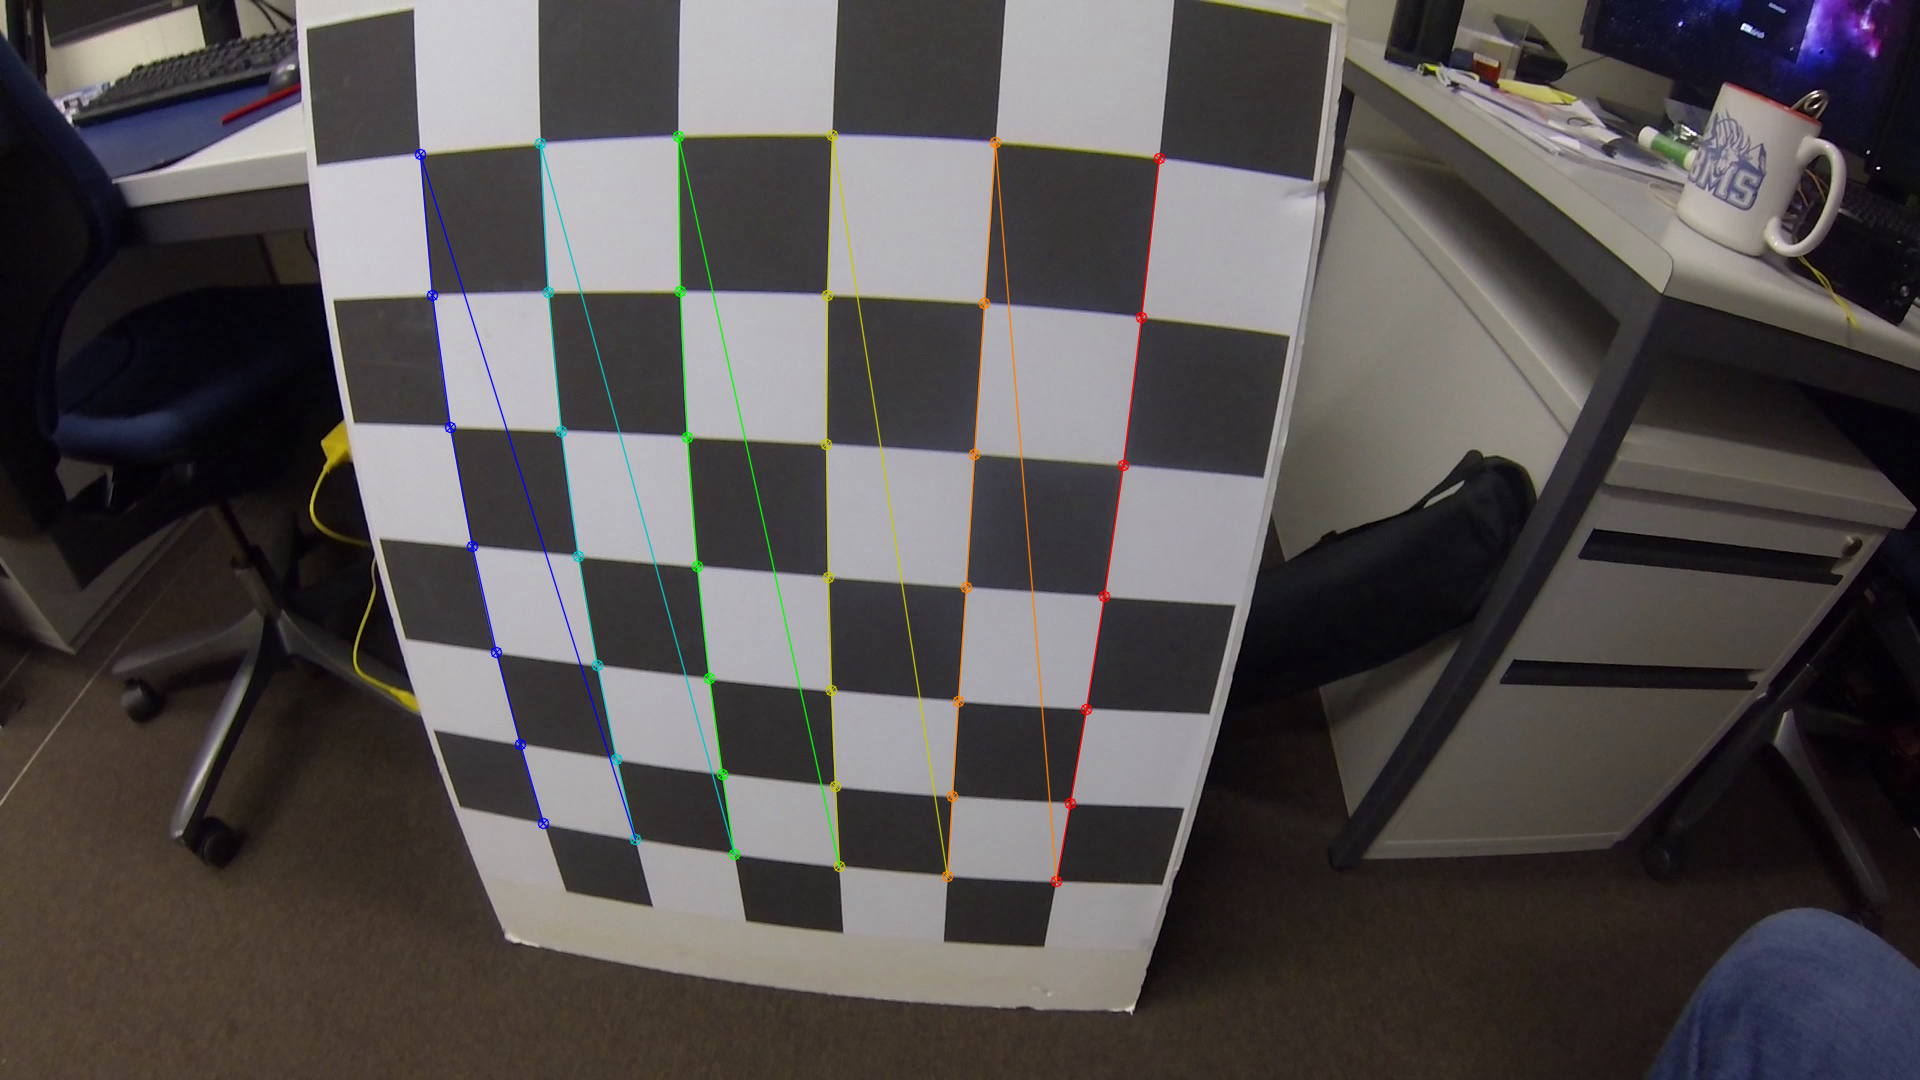
\includegraphics[width=0.75\textwidth]{../plots/intrinsic_calibration/gopro3_first_detection.png}
    \caption{Example of the chessboard corners detected in the gopro3 camera}
    \label{fig:chessboard_detection}
\end{figure}

\subsection{Drone Detection}

The first step for the 3D trajectory reconstruction is to detect the drone in each frame of the videos.\\

Initially, the drone was detected using a classical background subtraction method. We applied a Gaussian Mixture-based background subtractor (MOG2) to isolate moving objects against a mostly static sky background. After noise filtering with morphological operations, we analyzed contours in the foreground mask and filtered drone candidates based on area, aspect ratio, and vertical position constraints. Among these, the best candidate was selected either by spatial continuity (if a previous position was known) or by maximum area. To reduce jitter and improve stability, the detected positions were smoothed over time using a weighted average with the recent tracking history. This approach worked well when the drone was clearly visible and motion was distinct, but it became unreliable in the presence of occlusions, intermittent visibility, or when the drone was stationary.\\

To improve robustness, especially during frames where the drone was not clearly visible or briefly occluded, we integrated optical flow tracking using the Lucas-Kanade method. After an initial detection via background subtraction, we initialized tracking by identifying good features within the drone's bounding box. Between consecutive frames, these features were tracked to estimate the drone's displacement, allowing us to update its position even in the absence of fresh detections. We incorporated validation checks to assess confidence in the optical flow results and fall back to background subtraction when necessary. This hybrid approach significantly enhanced the continuity and accuracy of the trajectory, particularly during challenging segments of the video sequence, and reduced the frequency of detection failures.

\begin{figure}[H]
    \centering
    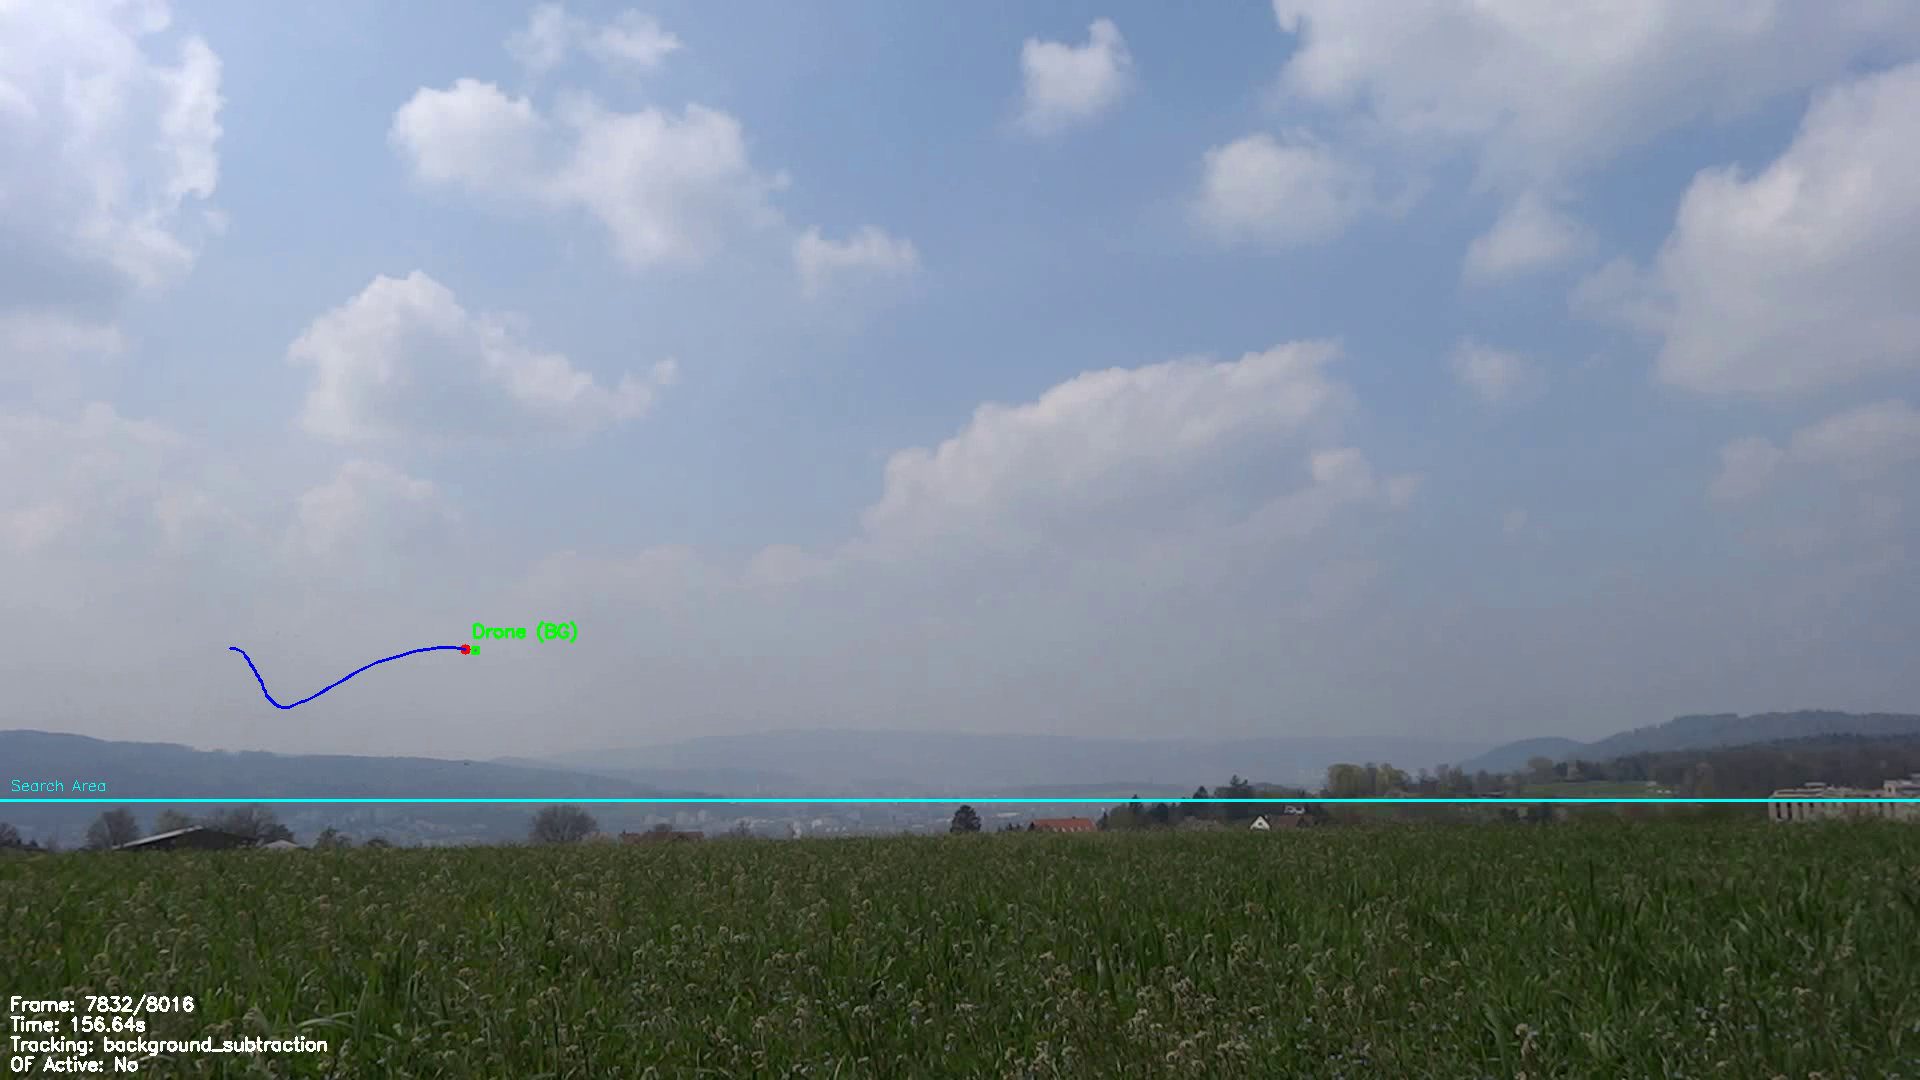
\includegraphics[width=.75\textwidth]{imgs/drone_detection_bs.png}
    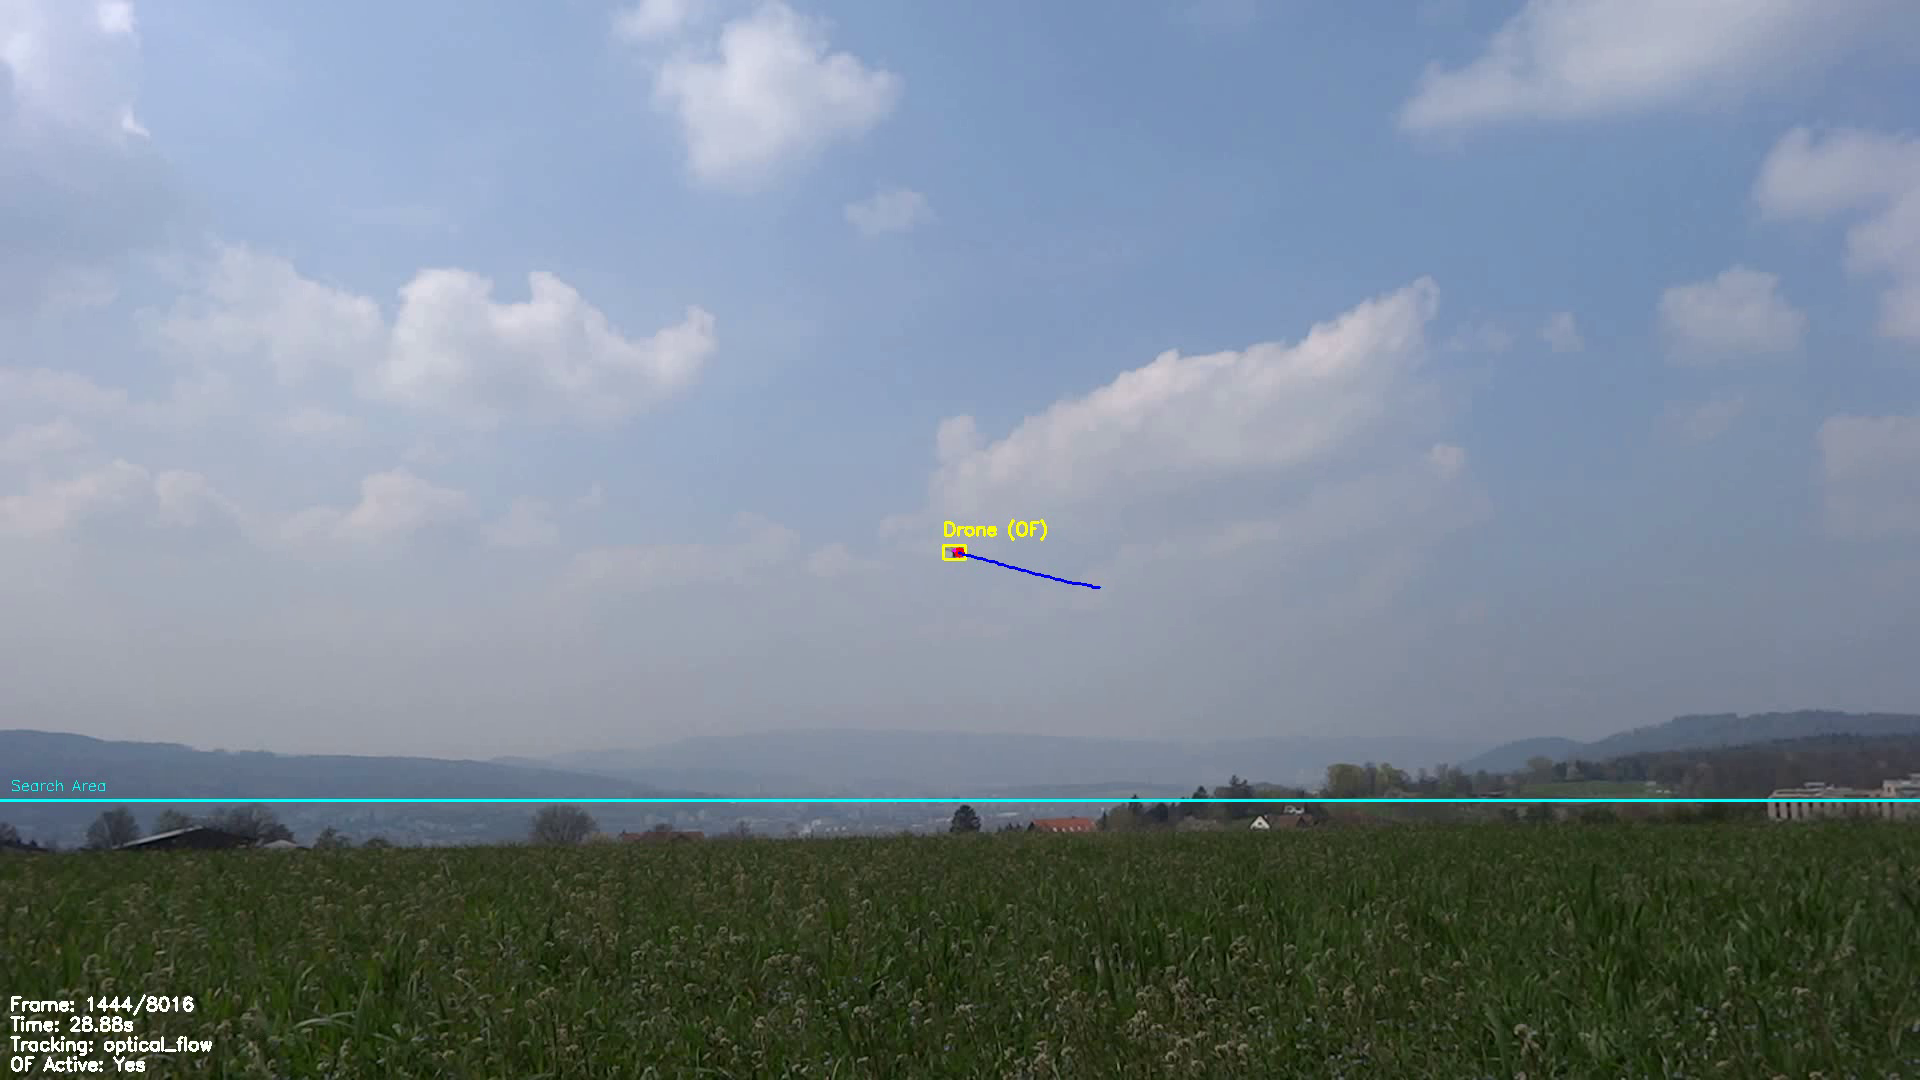
\includegraphics[width=.75\textwidth]{imgs/drone_detection_of.png}
    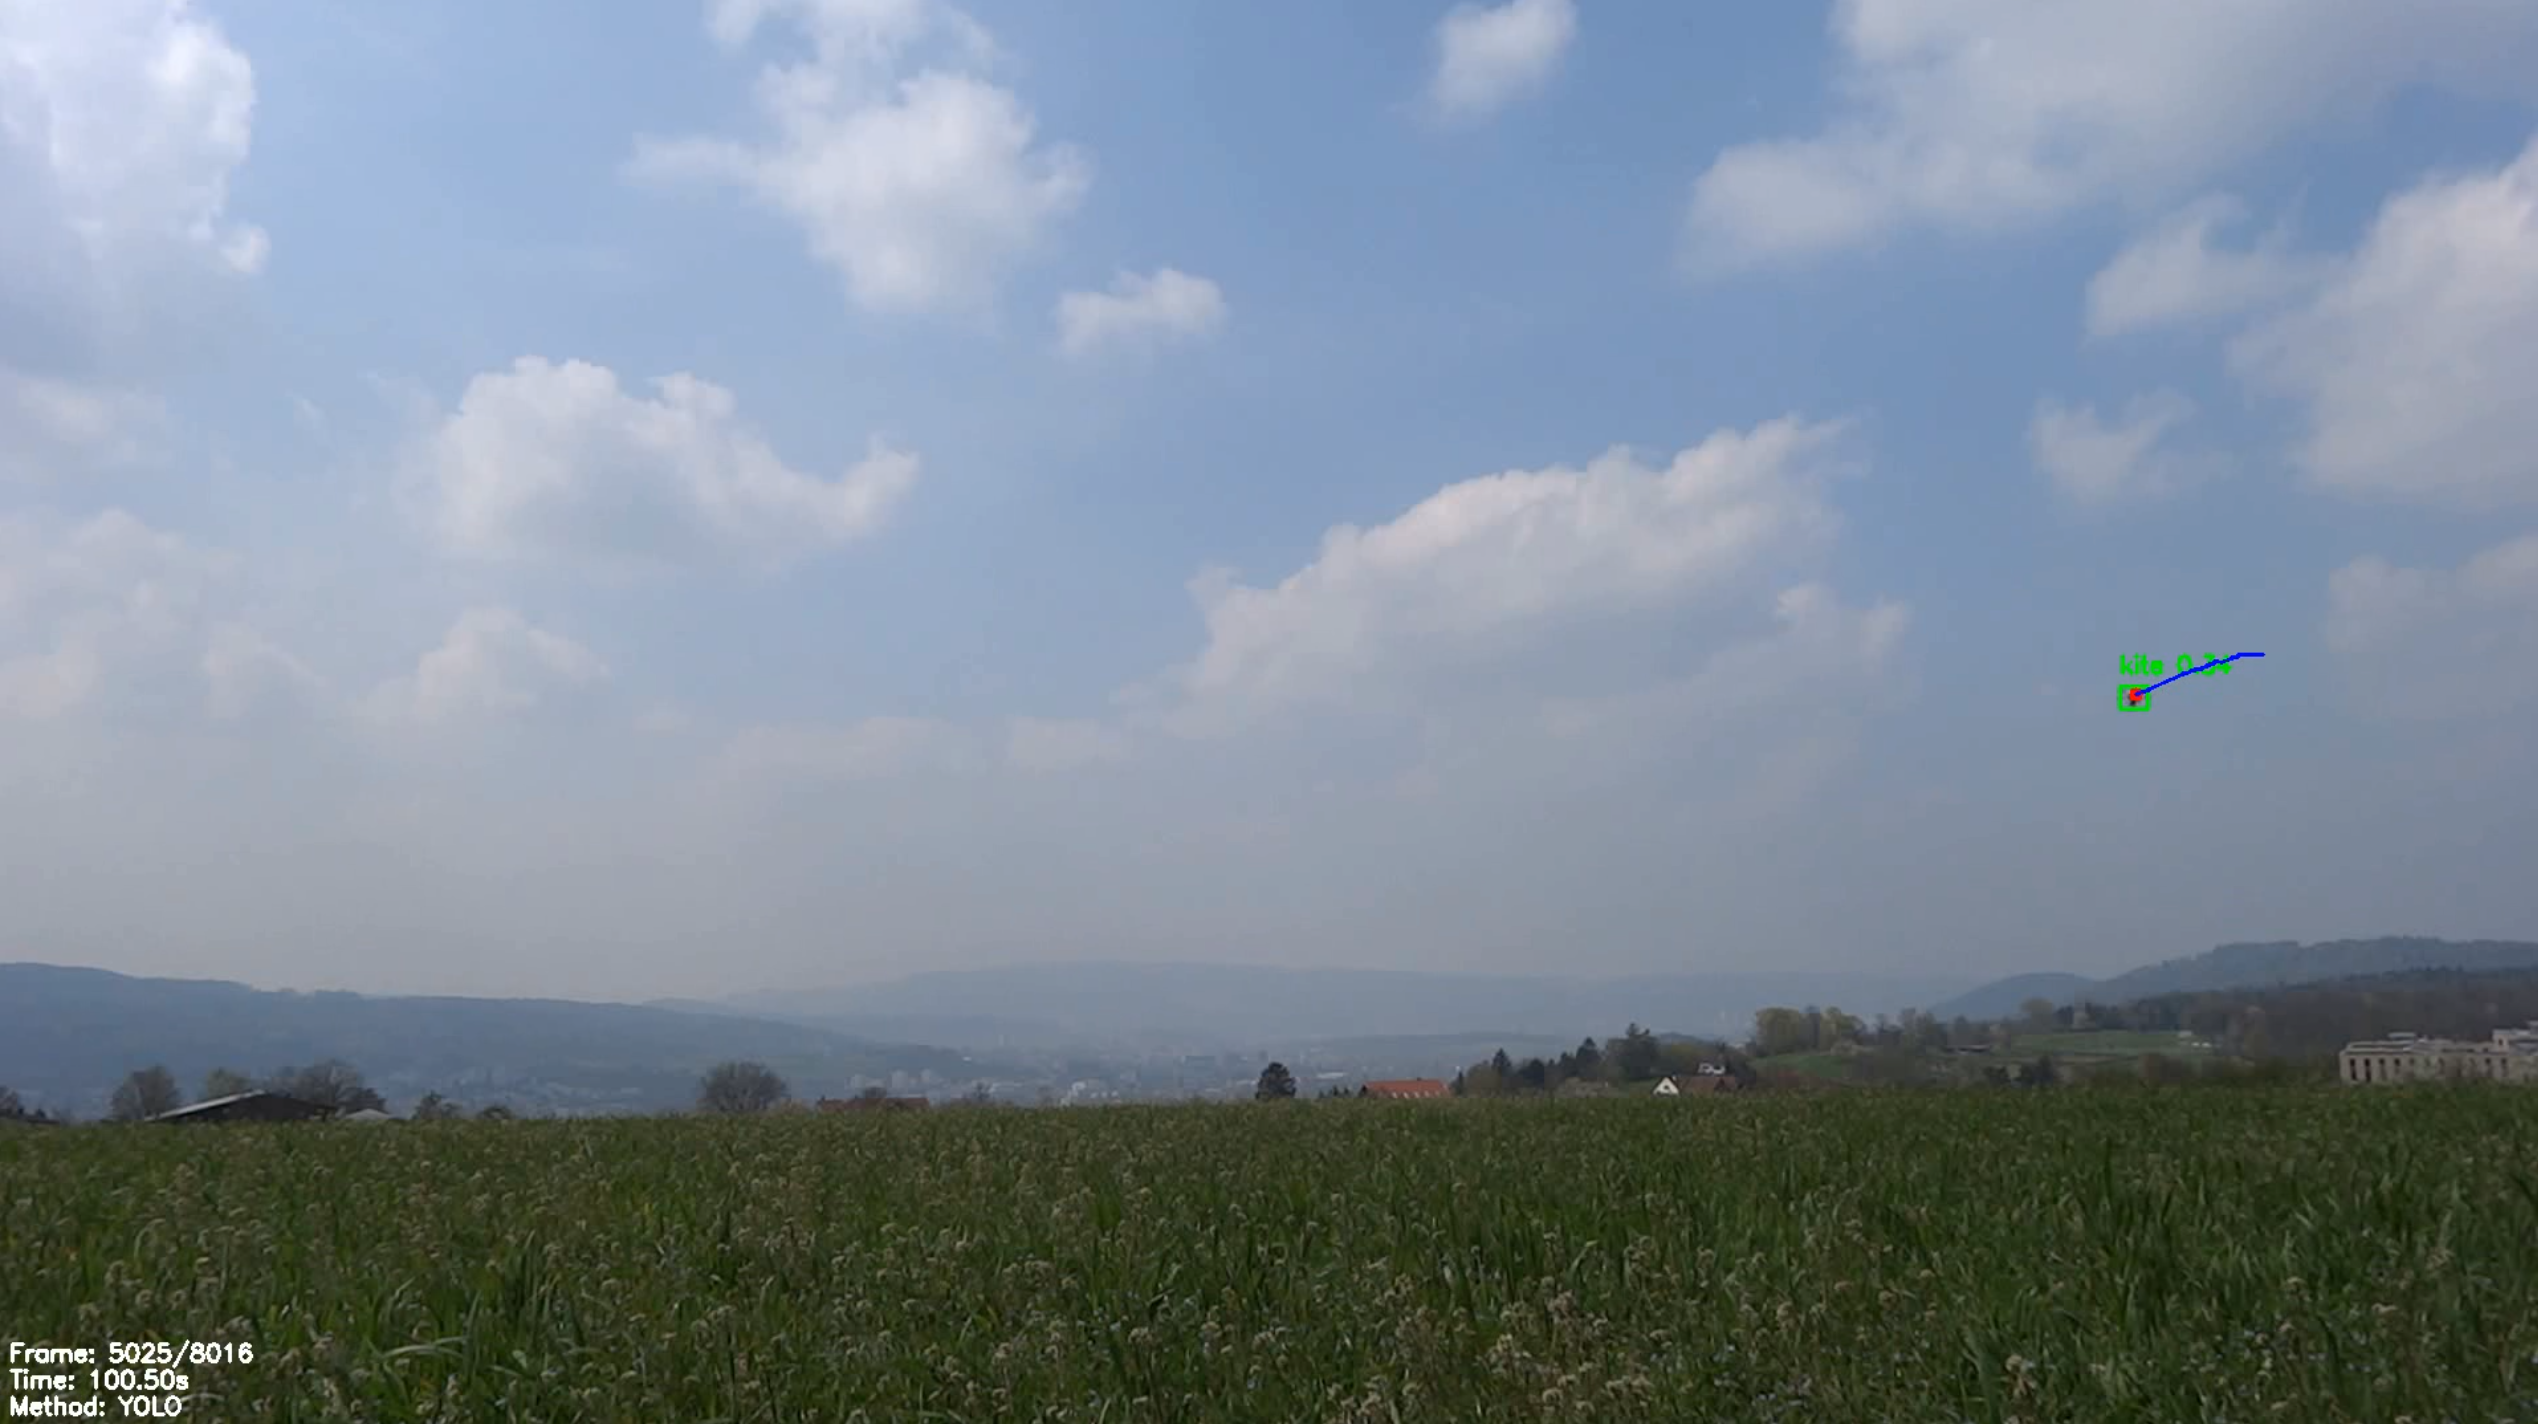
\includegraphics[width=.75\textwidth]{imgs/drone_detection_yolo.png}
    \caption{Frames taken from the result of the drone detection background subtraction (top), optical flow tracking (middle), and YOLOv8 (bottom)}
    \label{fig:drone_detection}
\end{figure}

To achieve this result, it is also possible to use a deep learning-based object detection algorithm, such as YOLO or SSD, that could give better results in terms of accuracy and robustness. We decided to use YOLOv8, which is a state-of-the-art object detection algorithm. We used the pre-trained weights provided by the \texttt{yolov8n}, which is a small and fast version of YOLOv8, without fine tuning.

\subsubsection*{Results}
\label{sec:drone_detection_results}

The drone detection algorithm was evaluated on some videos from the dataset, and the results were imperfect but promising. The main limitations were:

\begin{itemize}
    \item In the majority of the frames, the algorithm identified the partially visible grass as the drone, because it was moved by the wind. This problem was mitigated by applying a threshold on the area of the detected object, to be set for each video (light blue line in Figure \ref{fig:drone_detection})
    \item The algorithm often mistook the drone for other moving objects in the scene, such as birds. Unfortunately, this problem could not be solved, as the drone was often too small in the frame to be distinguished from other objects. To partially mitigate this issue, we saved also the velocity of the detected object for each frame (as shown in \ref{fig:detection_plots}), and we think that this information could be used to filter out false positives
    \item The deep learning-based detection algorithm completely removed the false positives, but it was not able to detect the drone in some frames, especially when the drone was too small in the frame, as shown in Figure \ref{fig:yolo_analysis}
\end{itemize}

\begin{figure}[H]
    \centering
    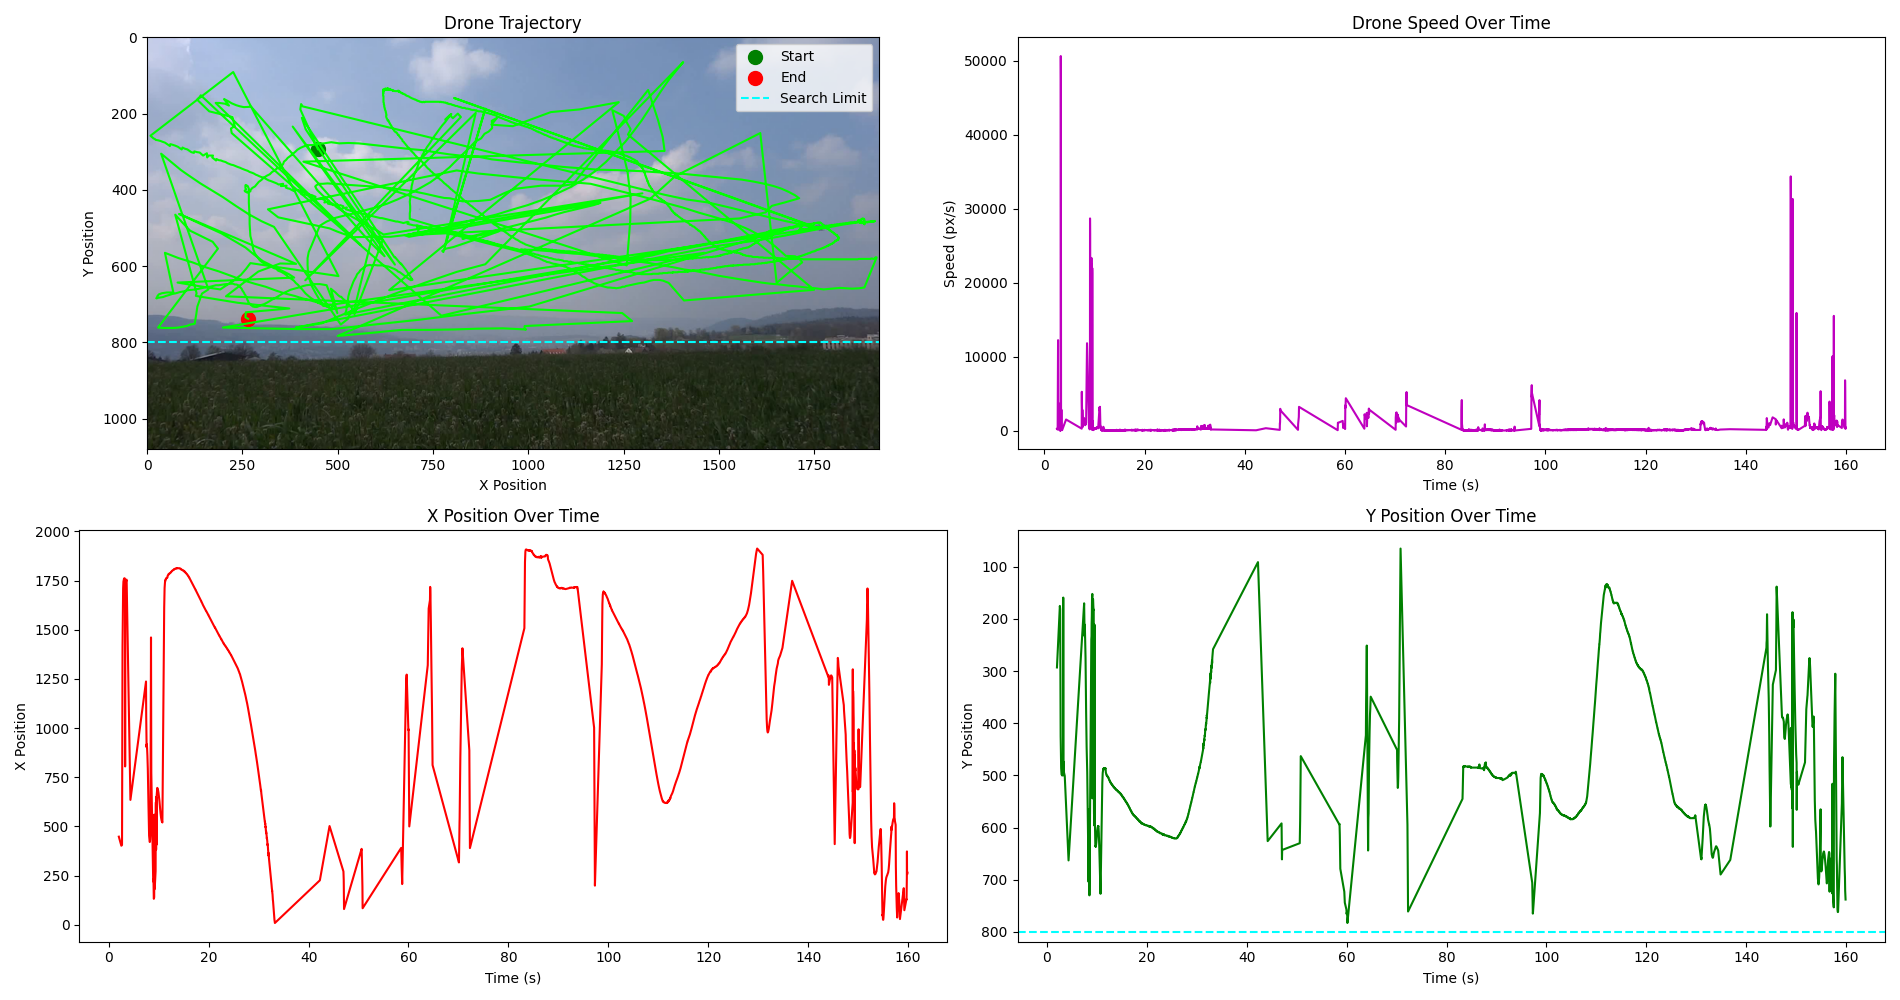
\includegraphics[width=\textwidth]{imgs/drone_tracking_output_trajectory.png}
    \caption{Analysis of the drone detection algorithm on a video from the dataset (Dataset 1, cam 2). It is clear the heavy presence of false positives, as the algorithm often detects birds and other moving objects as the drone. The velocity of the detected object is also shown, which could be used to filter out false positives.}
    \label{fig:detection_plots}
\end{figure}

\begin{figure}[H]
    \centering
    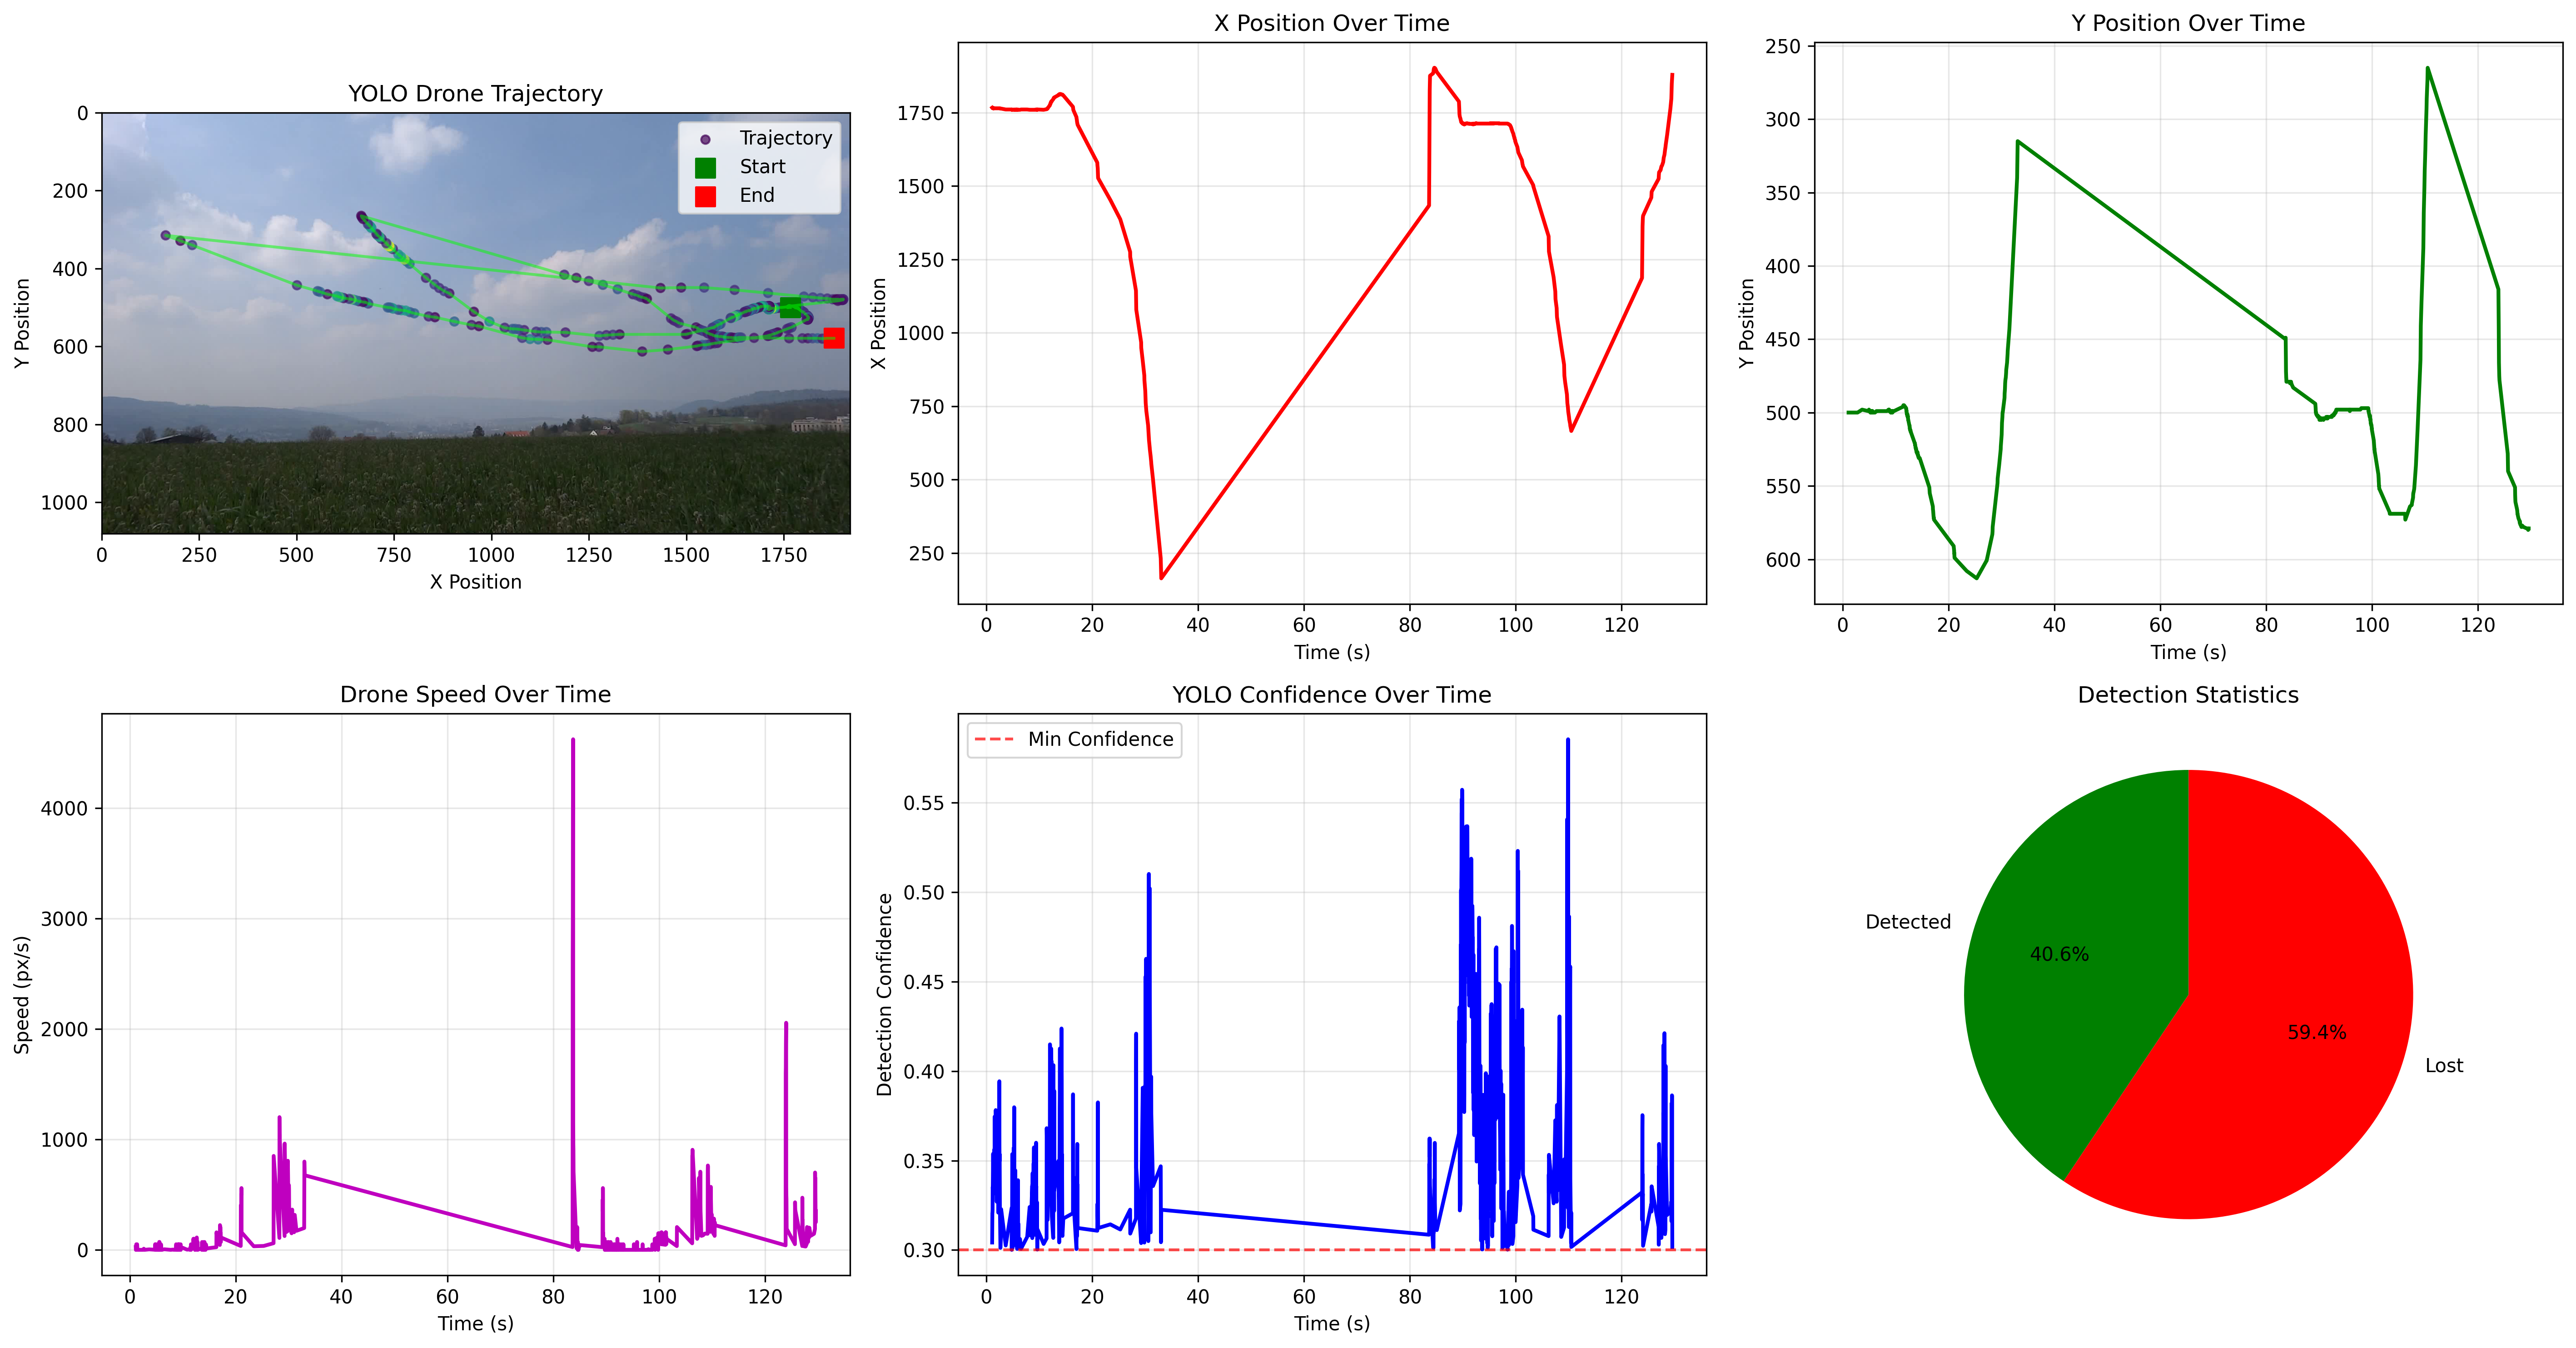
\includegraphics[width=\textwidth]{imgs/yolo_analysis.png}
    \caption{Analysis of the drone detection algorithm using YOLOv8 on a video from the dataset (Dataset 1, cam 2)}
    \label{fig:yolo_analysis}
\end{figure}

Due to the limitations of the detection algorithm, we decided to use the drone detections already given in the dataset. This allowed us to focus on the trajectory reconstruction aspect of the project.

\subsection{Offline Trajectory Reconstruction}

The next step was to reconstruct the drone's trajectory by loading all the detections in memory and then applying the reconstruction algorithm.

\subsubsection{Data loading}
\label{sec:data_loading}

The first step was to load the drone detections from the dataset. The dataset provides the drone detections in various \texttt{txt} files, divided in the repo by dataset and camera. Each \texttt{txt} file was automatically fetched and parsed, extracting the drone detections and frame indexes. In order to correctly handle the data and perform all the necessary operations, we decided to undistort the drone detections using the intrinsic parameters provided in the dataset at this stage. The intrinsic parameters were loaded from the calibration files provided in the dataset, and the drone detections were undistorted using OpenCV's \texttt{undistortPoints} function.

The undistorted drone detections were then saved in a \texttt{csv} file, unique for each dataset, with the same columns as the original \texttt{txt} files (frame index, x coordinate, y coordinate) with the addition of the camera index. This allowed us to easily access the drone detections for each camera and perform the necessary operations on them, both in the offline and online trajectory reconstruction algorithms.

\subsubsection{Temporal shift estimation}

One of the main goals in the paper is to have a system that does not require any synchronization between the cameras. This means that the timestamps of the frames are not aligned, and we needed to find the best temporal shift and scale factor between the cameras to align the drone detections.

following the paper notation, we can label each detection $j$ in each camera $i$ with a timestamp

\begin{equation}
    t_i^j = \alpha_i j + \beta_i
\end{equation}

Where $\beta_i$ is an offset and $\alpha_i$ is a scale factor which toghether map the frame index $j$ to a global time (or, equivalently, to the frame index of a reference camera $k$ such that $t_k^j = j$).

To estimate the temporal offsets ($\beta$) and scale factors ($\alpha$) between cameras, we implemented a straightforward algorithm that performs a brute-force search for the optimal temporal shift for each camera pair. The relative frame rate between cameras is imposed by setting the scale factor as the ratio of their respective frame rates.

For each candidate value of $\beta$ within a specified range, the algorithm shifts the detections of one camera accordingly and computes the fundamental matrix \textit{F} between the two cameras using the available drone detections as point correspondences. \textit{F} is estimated via RANSAC, and the number of inliers serves as a score to assess the quality of the temporal alignment. To refine the estimate, the search is repeated iteratively: after each iteration, the best $\beta$ is used to define a narrower and finer search range, and this process is repeated for four iterations.

An example of the results of this algorithm is shown in Figure \ref{fig:beta_search}

\begin{figure}[h]
    \centering
    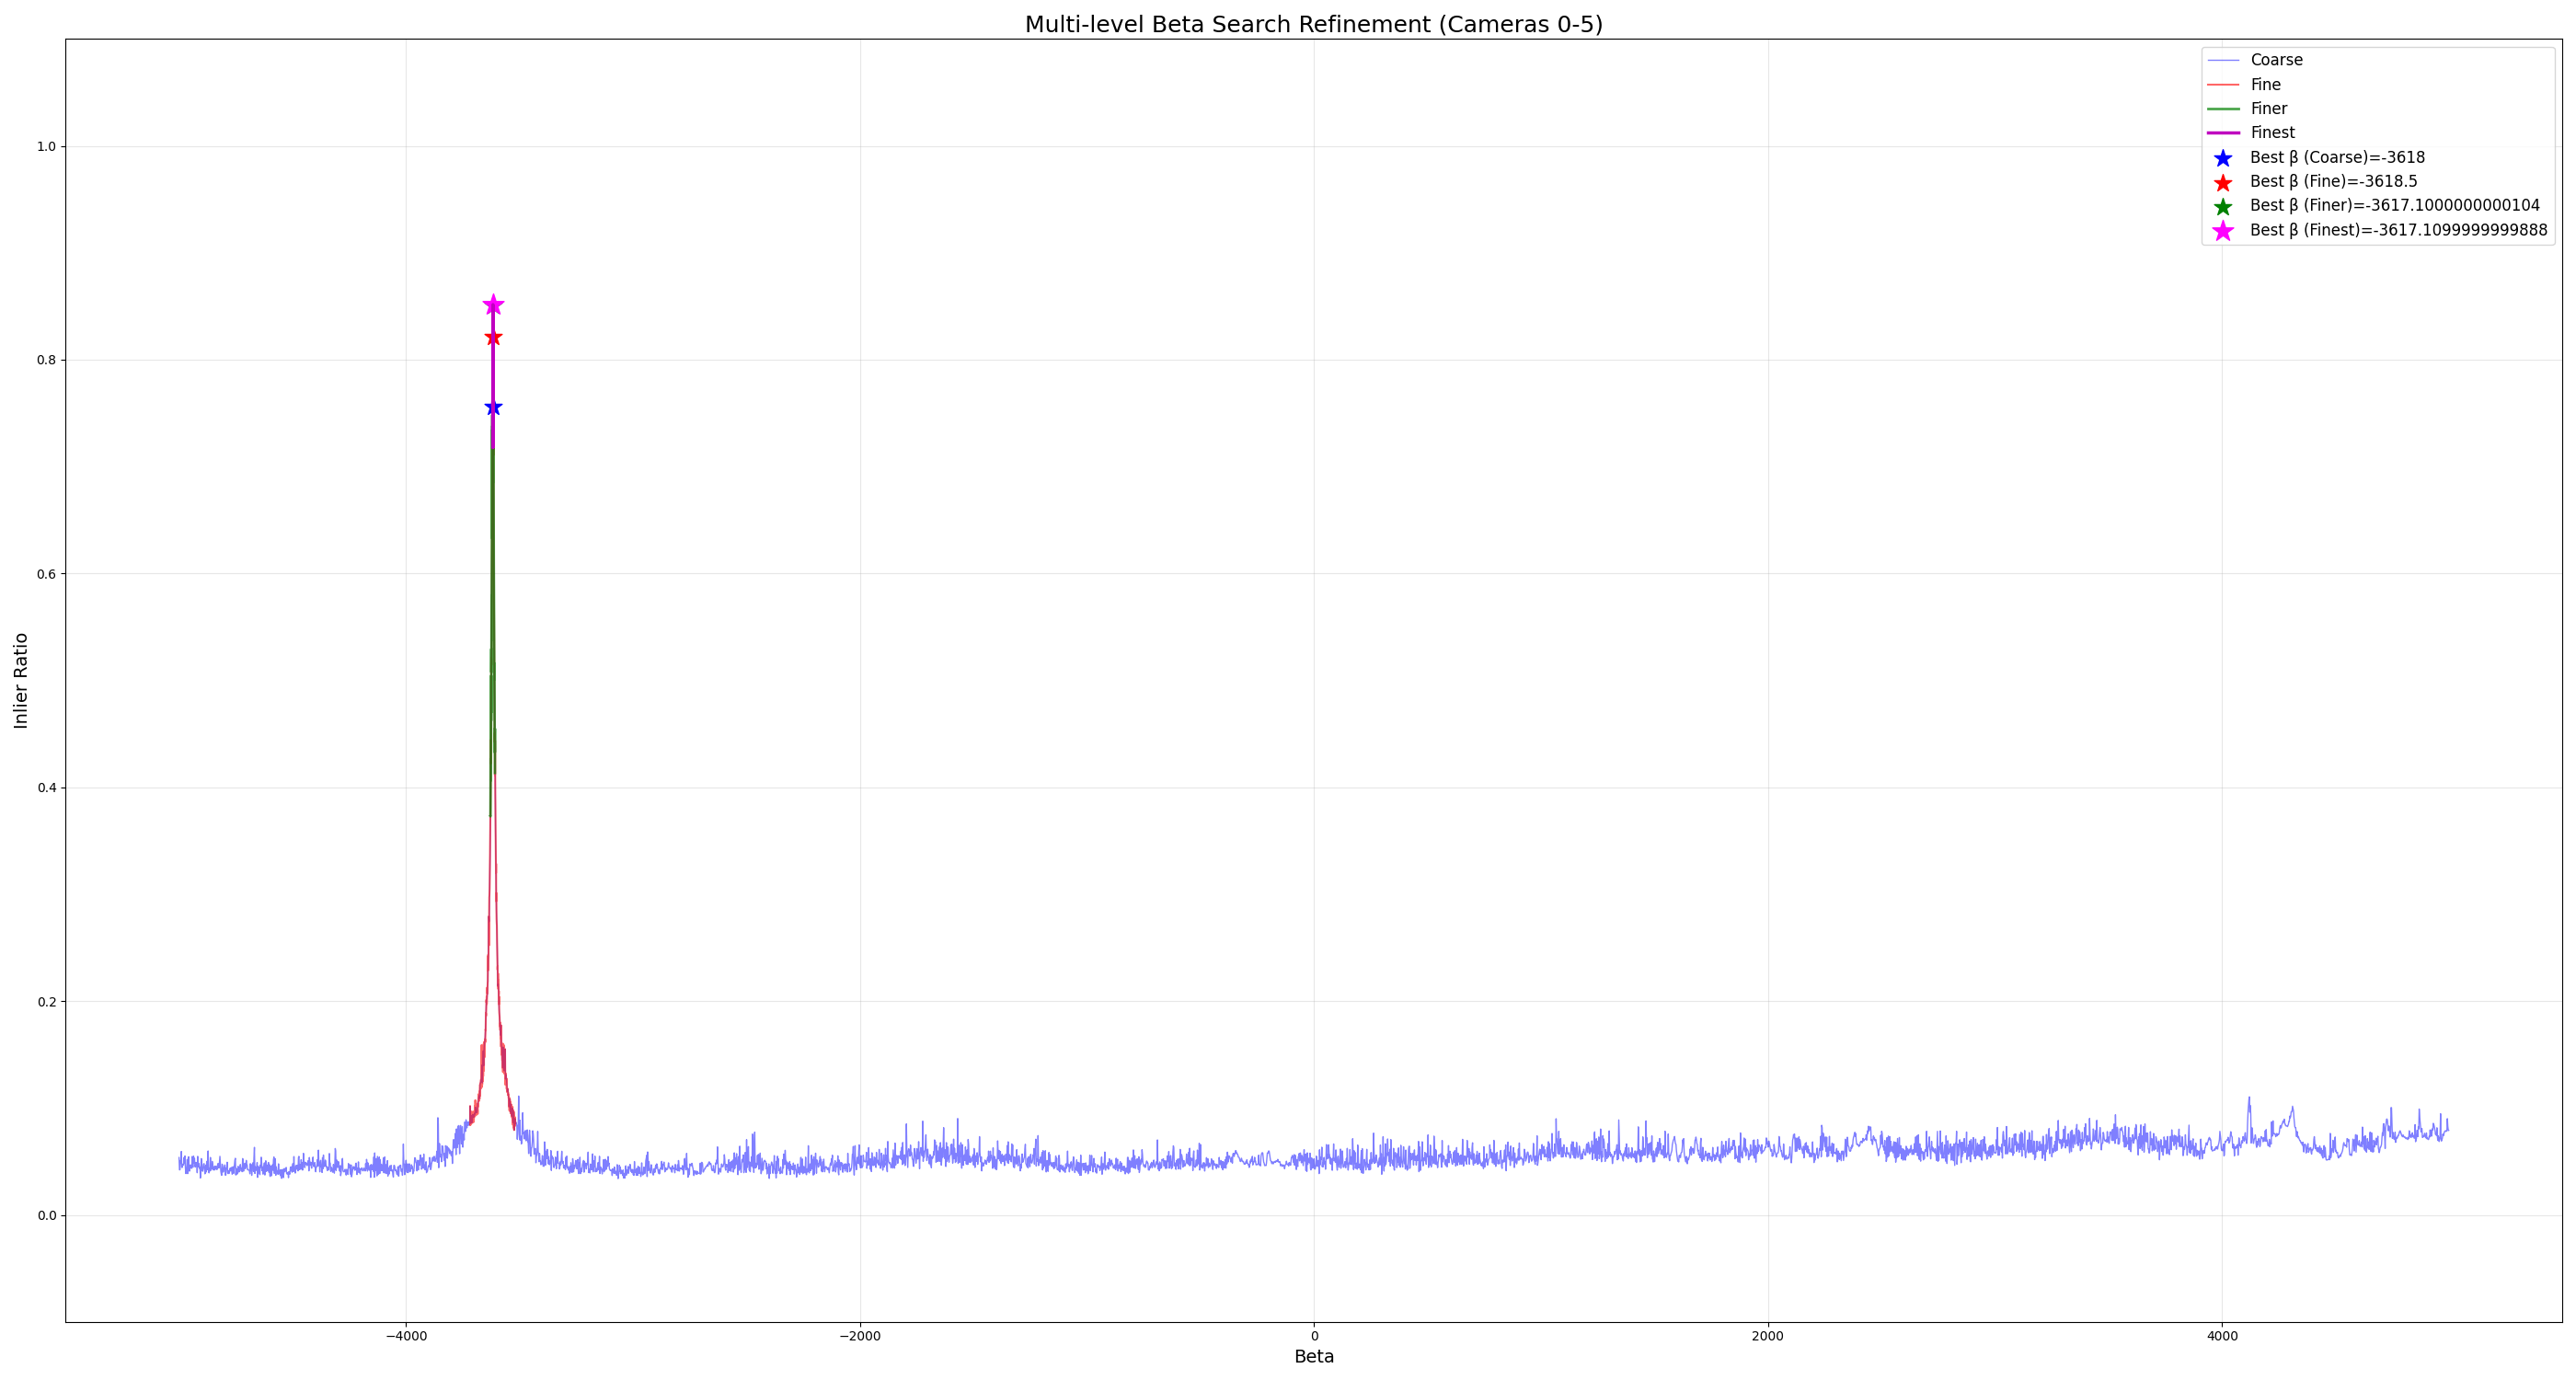
\includegraphics[width=\textwidth]{../plots/search_results/dataset4/inliers_vs_beta_combined_cam0-5_ds4.png}
    \caption{Example of the results of the temporal shift estimation algorithm (dataset 4, cameras 0-5). The x-axis shows the temporal shift $\beta$ in seconds, while the y-axis shows the number of inliers found for each candidate value of $\beta$. It is clear that the algorithm finds a peak in the number of inliers for a specific value of $\beta$, which is the best temporal shift between the two cameras.}
    \label{fig:beta_search}
\end{figure}

To establish correspondences between cameras, we adopted the approach described in the paper: for each detection in camera $i$, we search for a temporally overlapping set of consecutive detections in camera $j$ (after applying the current temporal shift). If such an overlap exists, we fit a spline to the detections in camera $j$ and evaluate it at the timestamp of the detection in camera $i$. This provides a set of matched points that can be used to compute \textit{F}\footnote{In order to decrease the computational effort, we decided to pre-compute and save all 2D splines only once, and then shift the timestamps when needed}.

This method, while simple, proved effective for aligning the detections across unsynchronized cameras and enabled robust estimation of the temporal shifts required for subsequent trajectory reconstruction.

From then on, each camera pair was processed in order of decreasing number of inliers, so that the cameras with the most reliable detections were processed first. This was done to ensure that the trajectory reconstruction was as accurate as possible.

\subsubsection{First camera pose estimation}

We started the trajectory reconstruction by estimating the relative pose of the best camera pair, which was the one with the most inliers in the estimation of \textit{F}. We referred to the camera whose detections had been interpolated with the spline as the \texttt{main\_camera} (\textit{mc}), and the other one as the \texttt{secondary\_camera} (\textit{sc}).

The following step was to compute the essential matrix \textit{E}. Since all the cameras were precalibrated, this could be done with the simple formula

\begin{equation}
    E = K_{mc}^T \cdot F \cdot K_{sc}
\end{equation}

Once we obtained \textit{E}, it was possible to recover the reciprocal pose of the two cameras thanks to OpenCV's function \texttt{cv.recoverPose}.

Since the relative positions could only be determined up to an unknown scale, we set the \texttt{main\_camera} pose at the origin with an identity rotation. All subsequent positions were then expressed relative to the baseline distance between these two cameras.

Once the 3D poses of the two cameras had been established, we could compute the projection matrices \texttt{P} for both cameras using the definition

\begin{equation}
    P = K \cdot [R | t]
\end{equation}

And, consequently, we used them to triangulate the 2D-2D correspondences, finding an initial set of 3D points.

\subsubsection{Other camera registration}

The process of registering additional cameras proceeded iteratively, selecting at each step the unregistered camera (\texttt{nth\_camera}, \textit{nc}) with the highest inlier ratio with respect to another in the set of already localized cameras (new \texttt{main\_camera}).

When a new couple was selected for localization, the same registration procedure was used: all 3D point and spline timestamps were mapped into the time frame of \textit{mc}, which then temporarily served as the global time reference for this step. For each detection in \textit{nc}, we searched for a temporally overlapping 3D spline and evaluated it at the timestamp of the detection in the camera. This provided a set of 3D-2D correspondences that could be used to localize \textit{nc} into the global frame using the PnP algorithm, with RANSAC employed to handle outliers.

\subsubsection{3D Splines extension}

Once each new camera was registered, we could extend the 3D splines to include the new detections. This was done by triangulating the new 2D-2D correspondences in the pair \textit{mc} - \textit{nc}, and then checking if the new 3D points extended the existing splines' time range. If they did, we extended the splines to include the new points, otherwise we simply added the new points to the existing splines. If a segment of new 3D points were able to bridge the gap between two existing splines, we merged the two splines into one. This was done to ensure that the 3D splines were as continuous as possible, and to avoid having too many small segments. This process is illustrated in Figure \ref{fig:3d_splines_extension}

\begin{figure}[H]
    \centering
    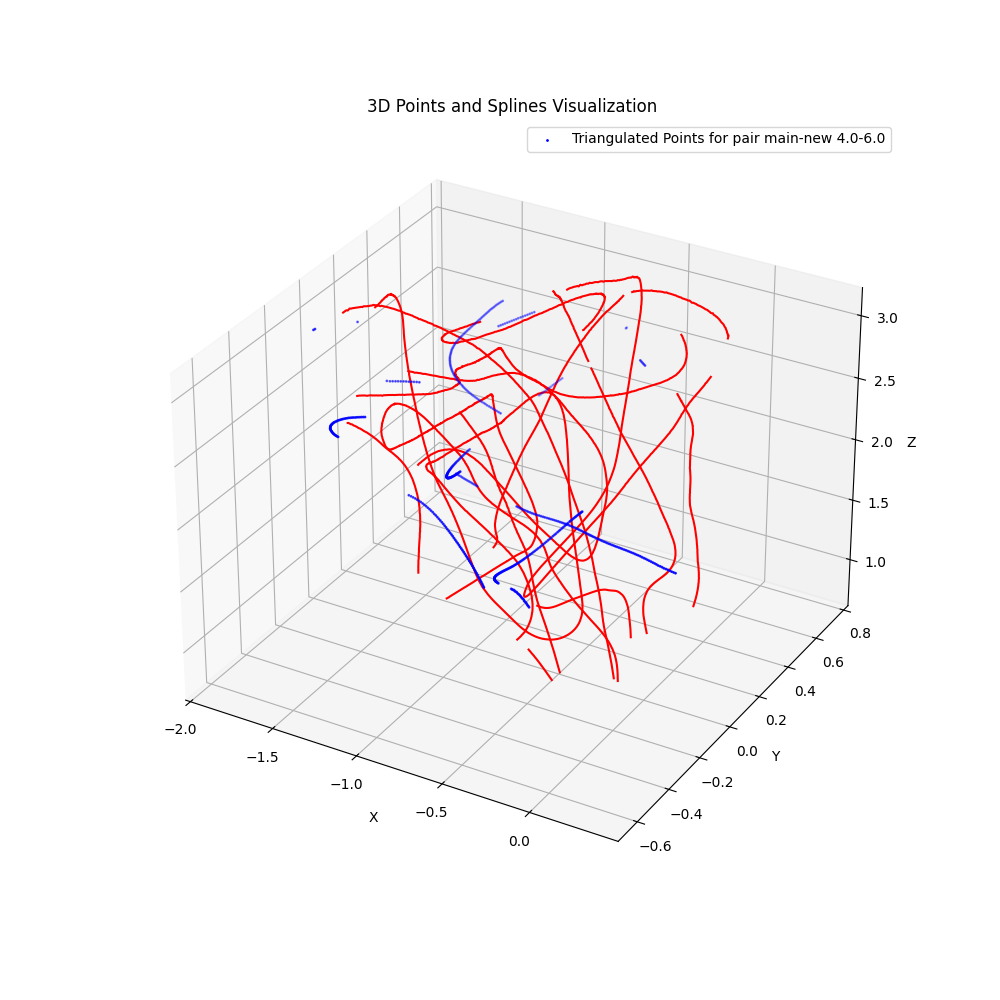
\includegraphics[width=.45\textwidth]{../plots/dataset4/Extension_to_splines_it2_4.0_6.0.png}
    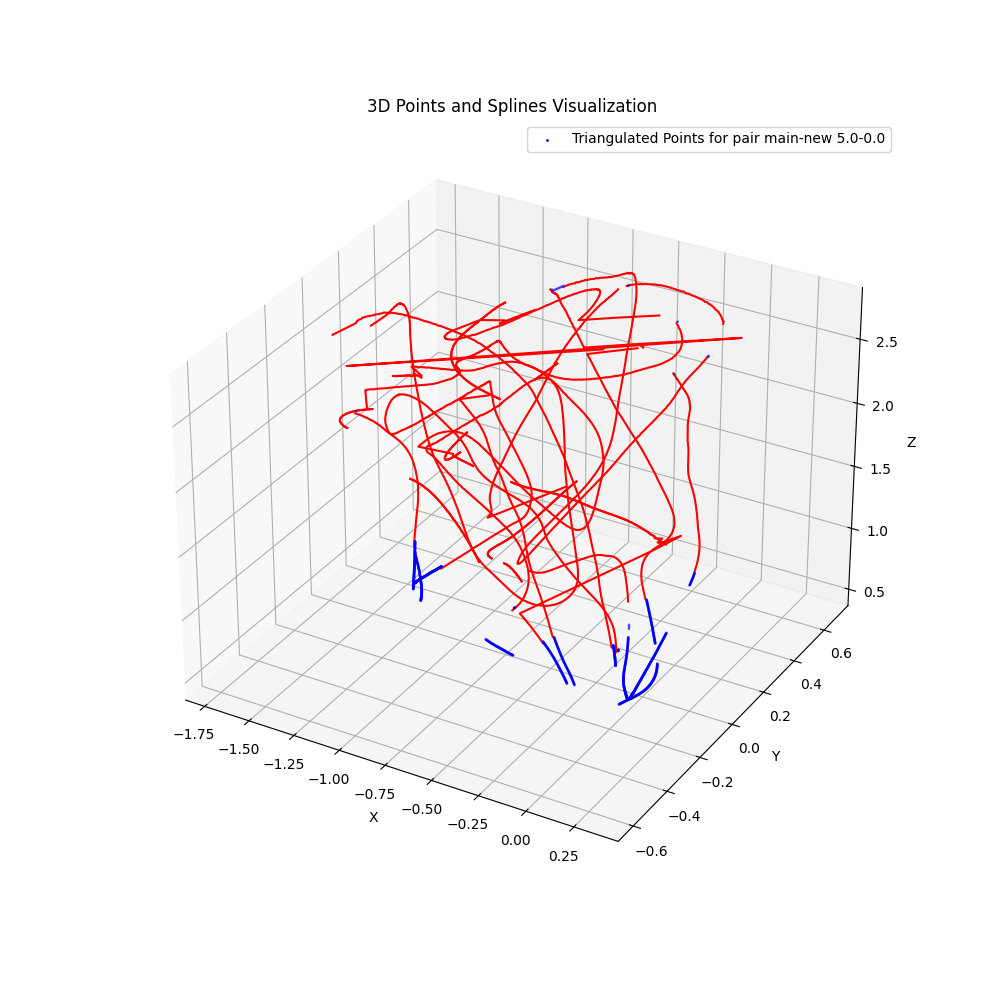
\includegraphics[width=.45\textwidth]{../plots/dataset4/Extension_to_splines_it3_5.0_0.0.png}
    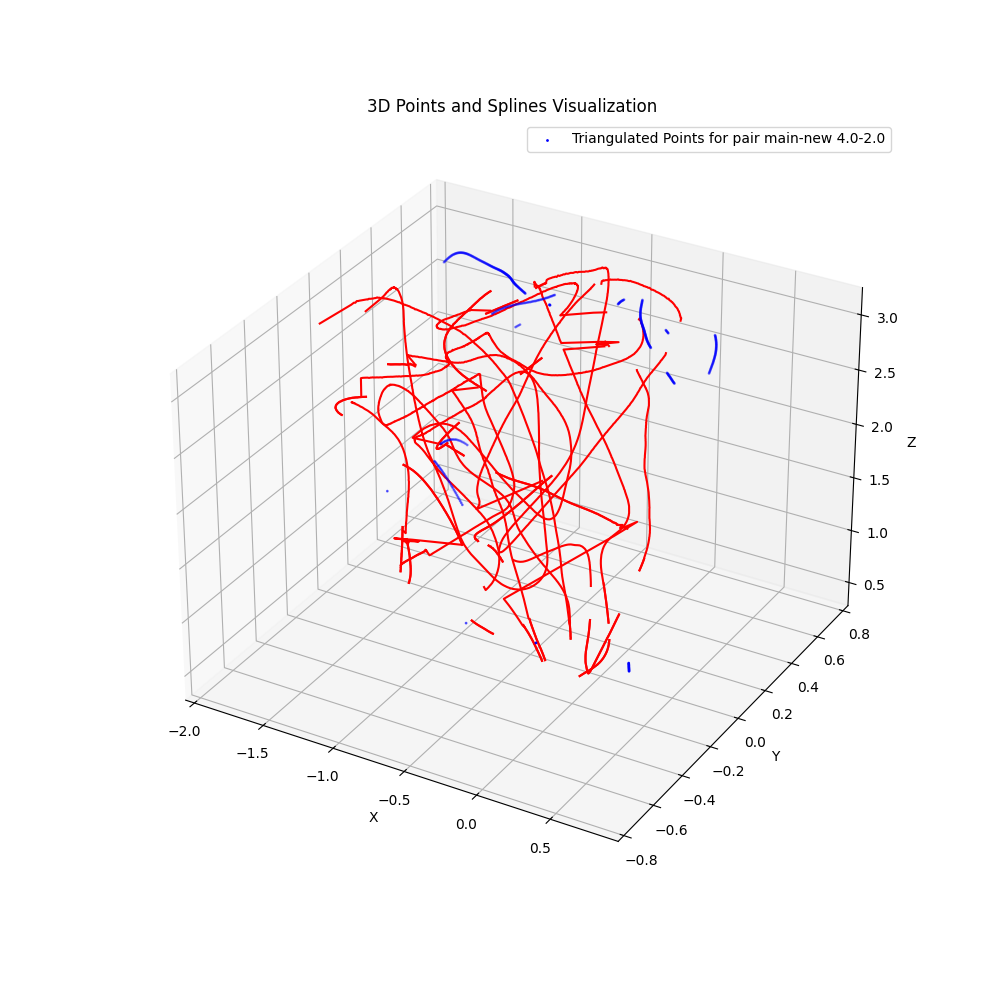
\includegraphics[width=.45\textwidth]{../plots/dataset4/Extension_to_splines_it4_4.0_2.0.png}
    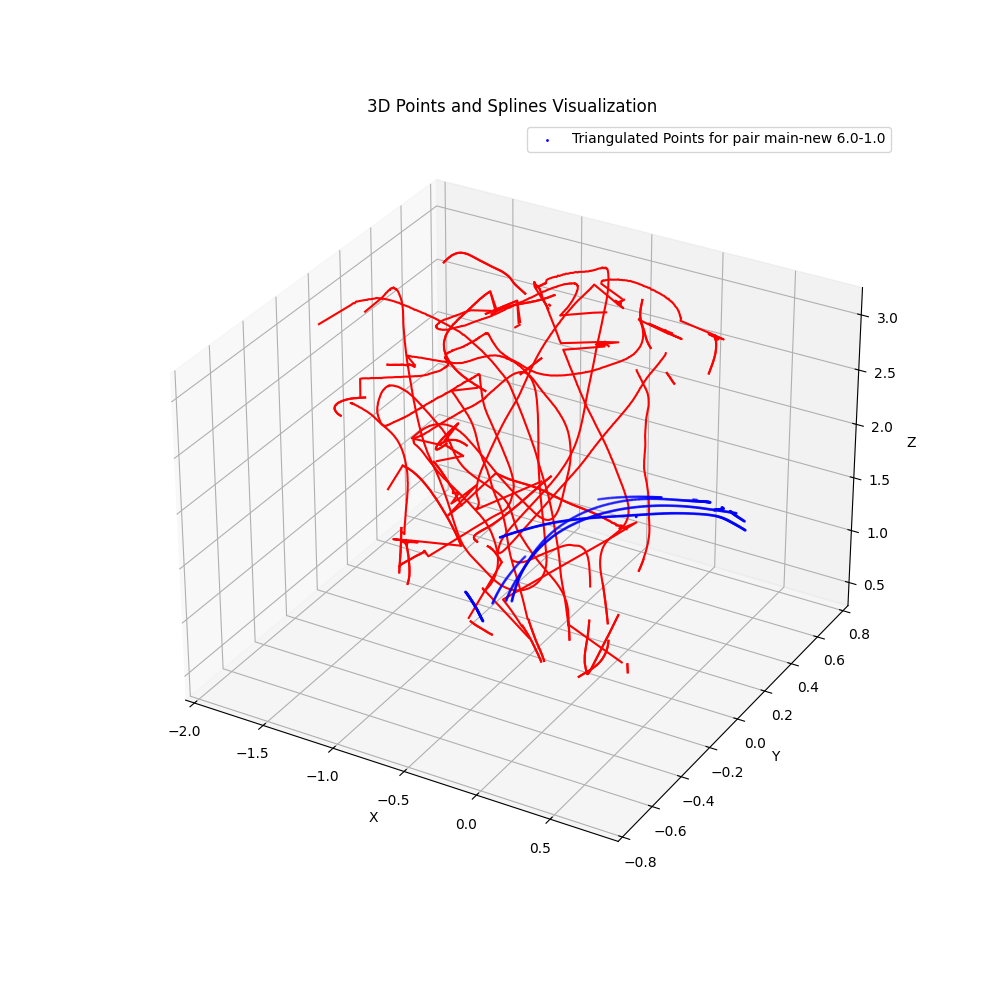
\includegraphics[width=.45\textwidth]{../plots/dataset4/Extension_to_splines_it5_6.0_1.0.png}
    \caption{Example of how the 3D splines are extended with the addition of new cameras (dataset 4). When a new camera is registered, the already existing 3D splines (red) are extended to include the new 3D points (blue)}
    \label{fig:3d_splines_extension}
\end{figure}

\subsubsection{Bundle Adjustment}

Since the procedure described above was prone to accumulate errors, we applied a bundle adjustment step to refine the 3D points and camera poses. This was done by interpolating the 3D splines at the timestamps of the detections in each camera, and then using the 2D-3D correspondences to minimize the reprojection error. The optimization was performed by Python's \texttt{scipy.optimize.least\_squares} function, which allowed us to minimize the error in a robust and efficient way. The effects of the bundle adjustment can be seen in Figure \ref{fig:reprojection_analysis}.

The bundle adjustment was performed for each registered camera every time a new camera was added.\\

After all cameras were registered, we should have had a complete 3D trajectory of the drone, with all cameras registered in the same global frame and all 3D points visible from at least two cameras. However, the implemented approach suffered from some limitations, that we are going to discuss in section \ref{sec:limitations}.

\subsection{Online Trajectory Reconstruction}

The paper also suggest the implementation of an online trajectory reconstruction algorithm, that is able to reconstruct the drone's trajectory in real-time as it flies.

\subsubsection{Environment and data loading}

In this case, we needed to simulate the stream of data from the cameras, as if it were coming from a real-time video feed. To do this, we choose to use ROS2 as the framework to handle the data stream, and we implemented a ROS2 node that receives the drone detections from every camera and reconstructs the trajectory in real-time.
To simulate a real-time data stream, we performed the following data preprocessing steps:
\begin{itemize}
    \item We loaded the drone detections from the \texttt{csv} file described in Section~\ref{sec:data_loading}.
    \item For each camera and each detection, we computed the global timestamp by applying the $\alpha$ and $\beta$ parameters provided in the dataset, ensuring robustness to timing inconsistencies.
    \item We sorted all detections by their global timestamps and created a list of messages to be stored in a ROS2 bag file.
\end{itemize}

\textbf{Note:} since in this approach we simulated the real-time data stream, we did not need to estimate the temporal shifts between cameras, as the timestamps were already aligned.\\

During the bag replay, all the logic for the trajectory reconstruction was implemented in a single ROS2 node, which subscribed to the drone detections.

\subsubsection{Data handling}

Since the data was received in real time, it was essential to handle the data stream efficiently. To achieve this, we implemented a subscriber that collected drone detections from each camera and stored them in a buffer. The buffer was organized as an array, where each element corresponded to a specific camera and contained a list of detections grouped by contiguous timestamps. This structure enabled fast access to the detections from each camera and made it easy to identify timestamp segments that were ready for spline interpolation without the need for repeatedly searching through the entire buffer.

\subsubsection{Cameras localization}

In order not to lose any incoming message during the trajectory reconstruction, all the logic for the camera localization and trajectory reconstruction was implemented in a separate thread. The tasks to be performed in this thread were the following:

After a sufficient number of detections had been collected in the buffer, the algorithm would find the correspondences between cameras and, if the number of correspondences between two cameras was sufficient, it would compute the fundamental matrix \textit{F}.

If \textit{F} brought to a sufficient number of inliers, the algorithm would compute the essential matrix \textit{E} and recover the relative pose of the two cameras in the same way as in the offline trajectory reconstruction.

After the relative pose of the two cameras was computed, the algorithm would generate the 3D positions of the drone by triangulating the 2D-2D correspondences between the two cameras, and then generate the initial 3D splines for the drone trajectory.

\begin{figure}[h]
    \centering
    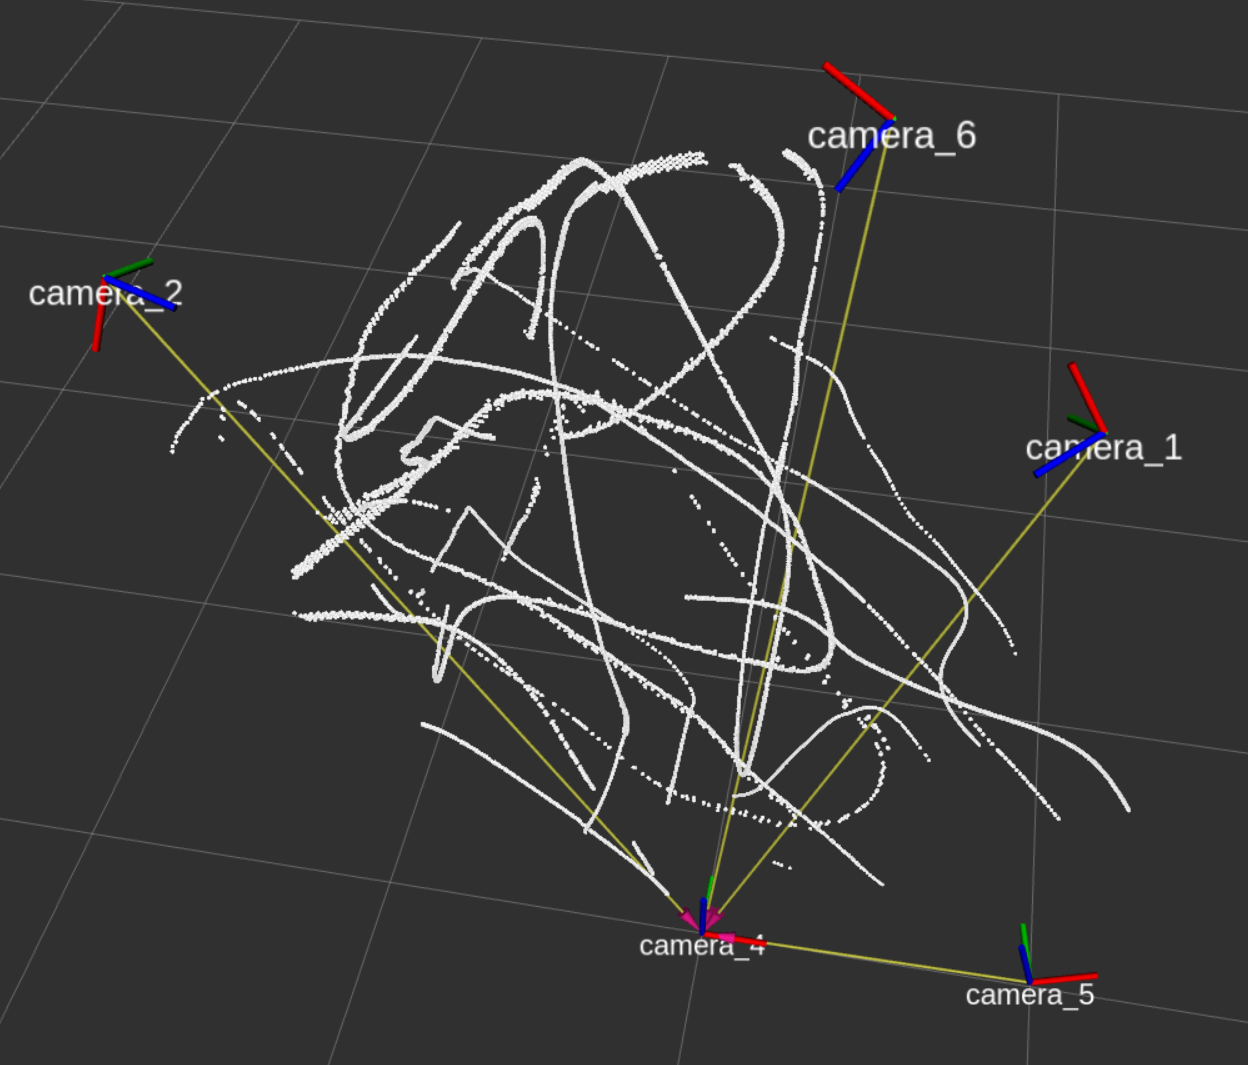
\includegraphics[width=0.6\textwidth]{imgs/online_full_trajectory.png}
    \caption{Example of the 3D trajectory reconstructed by the online algorithm (dataset 4). The drone positions are shown as white dots, while the cameras are shown as ROS tf frames}
    \label{fig:online_full_trajectory}
\end{figure}

Periodically, the algorithm would check if cameras not yet registered had enough correspondences with the 3D splines. If so, it would compute the relative pose of the new camera with respect to the global frame using the PnP algorithm

\subsubsection{3D Splines extension}

In parallel with the camera localization, the algorithm would also keep up to date the 3D trajectory of the drone in the following way:

\begin{itemize}
    \item For each new detection received from a camera $pc$, the algorithm would interpolate with a 2D spline the last 5 detections of the drone in $pc$ (if the detections were not too far apart in time)
    \item For every other camera $i$, if their last detection was within the 2D spline time range, the algorithm would evaluate the spline at the timestamp of the detection and generate a 2D-2D correspondence.
    \item Every correspondence $pc-i$ would be used to triangulate a 3D point, then these points would be averaged and added to the 3D splines of the drone trajectory.
    \item If the new 3D point was sufficiently close to last spline segment in time, the algorithm would extend the spline to include the new point.
\end{itemize}

This approach allowed the algorithm to keep the 3D trajectory of the drone up to date in real-time, while also registering new cameras as they became available.

\subsubsection{Bundle Adjustment}

As the paper suggested, the algorithm would periodically perform a bundle adjustment to refine the 3D trajectory of the drone and the camera poses. This was done in the same way as in the offline trajectory reconstruction (same code), and it was performed periodically (every 1000 detections) and in a separate thread to avoid blocking the main thread that was receiving the drone detections.

\section{Limitations of the implementation}
\label{sec:limitations}

The implemented pipeline, while functional, has several limitations that should be mentioned:

\subsection{Drone Detection}

The limitations of the drone detection algorithm were already discussed in Section \ref{sec:drone_detection_results}

\subsection{Offline Trajectory Reconstruction}

during the $\beta$ search phase, some of the smartphone cameras were recording at a variable frame rate. In some cases the fluctuation in FPS was very high, e.g. Mate 7 and Mate 10 in this dataset. For this reason, the algorithm was not able to find a peak in the number of inliers for these cameras, as shown in Figure \ref{fig:failed_beta_search}. This is because our implementation relies on the assumption that the frame rate is constant, and therefore it cannot handle cameras with variable frame rates.

The authors of the paper suggest to remap the detected points to a fixed frame rate with a linear interpolation, but we did not implement this step in our code. Instead, we simply ignored these cameras, as they were not essential for the trajectory reconstruction. An effect of this is shown in Figure \ref{fig:failed_beta_search}, where the algorithm fails to find a peak in the number of inliers for each camera pair including the above mentioned cameras.

\begin{figure}[h]
    \centering
    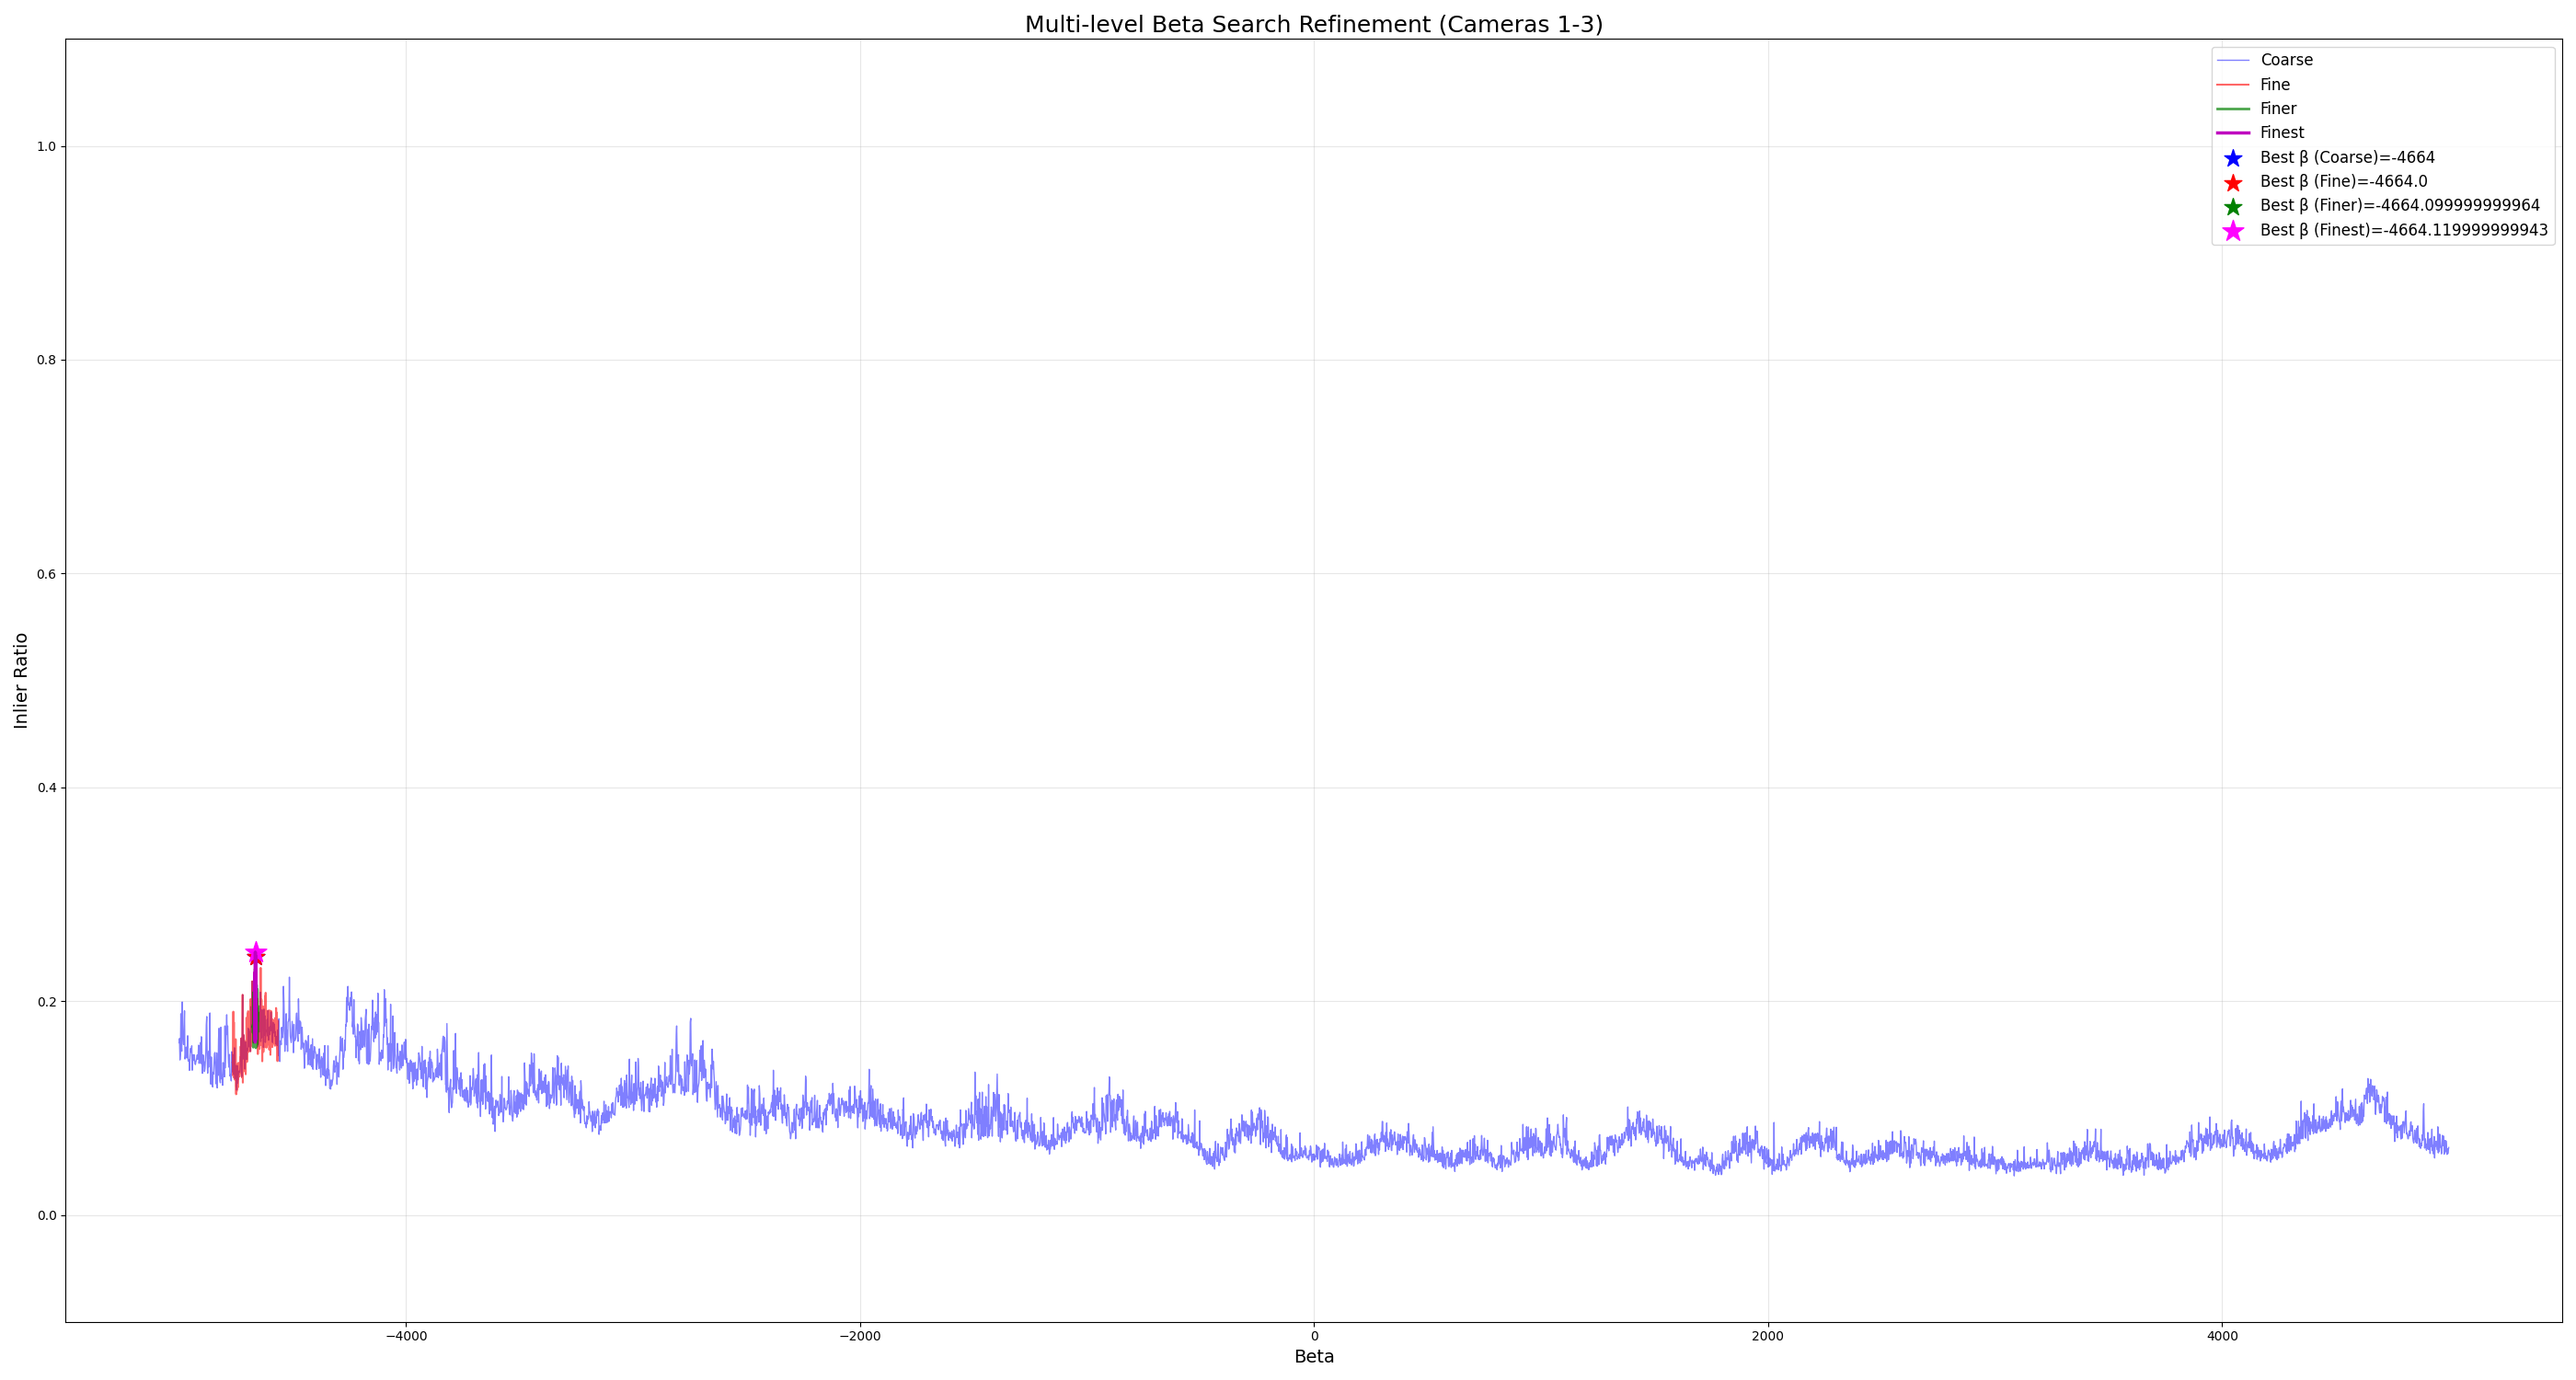
\includegraphics[width=\textwidth]{../plots/search_results/dataset4/inliers_vs_beta_combined_cam1-3_ds4.png}
    \caption{Example of the results of the temporal shift estimation algorithm (dataset 4, cameras 1-3). Due to the variable frame rate of the camera, the algorithm fails to find a clear peak in the number of inliers}
    \label{fig:failed_beta_search}
\end{figure}

Another limitation of the offline trajectory reconstruction is that the process of camera localization was prone to accumulating errors. As a result, when a new camera was registered, the 3D splines were not always continuous, and the reconstructed trajectory could be inaccurate. This led to temporal discontinuities in the splines, which in turn reduced the effectiveness of the bundle adjustment step. These issues are partially visible in Figure \ref{fig:reprojection_analysis}, where the bundle adjustment does not fully correct the reprojection errors. They are also evident in Figure \ref{fig:splines_discontinuity}, which shows discontinuous 3D splines and an imprecise trajectory, and in Figure \ref{fig:bad_ba}, where the bundle adjustment fails to refine the camera position.

\begin{figure}[h]
    \centering
    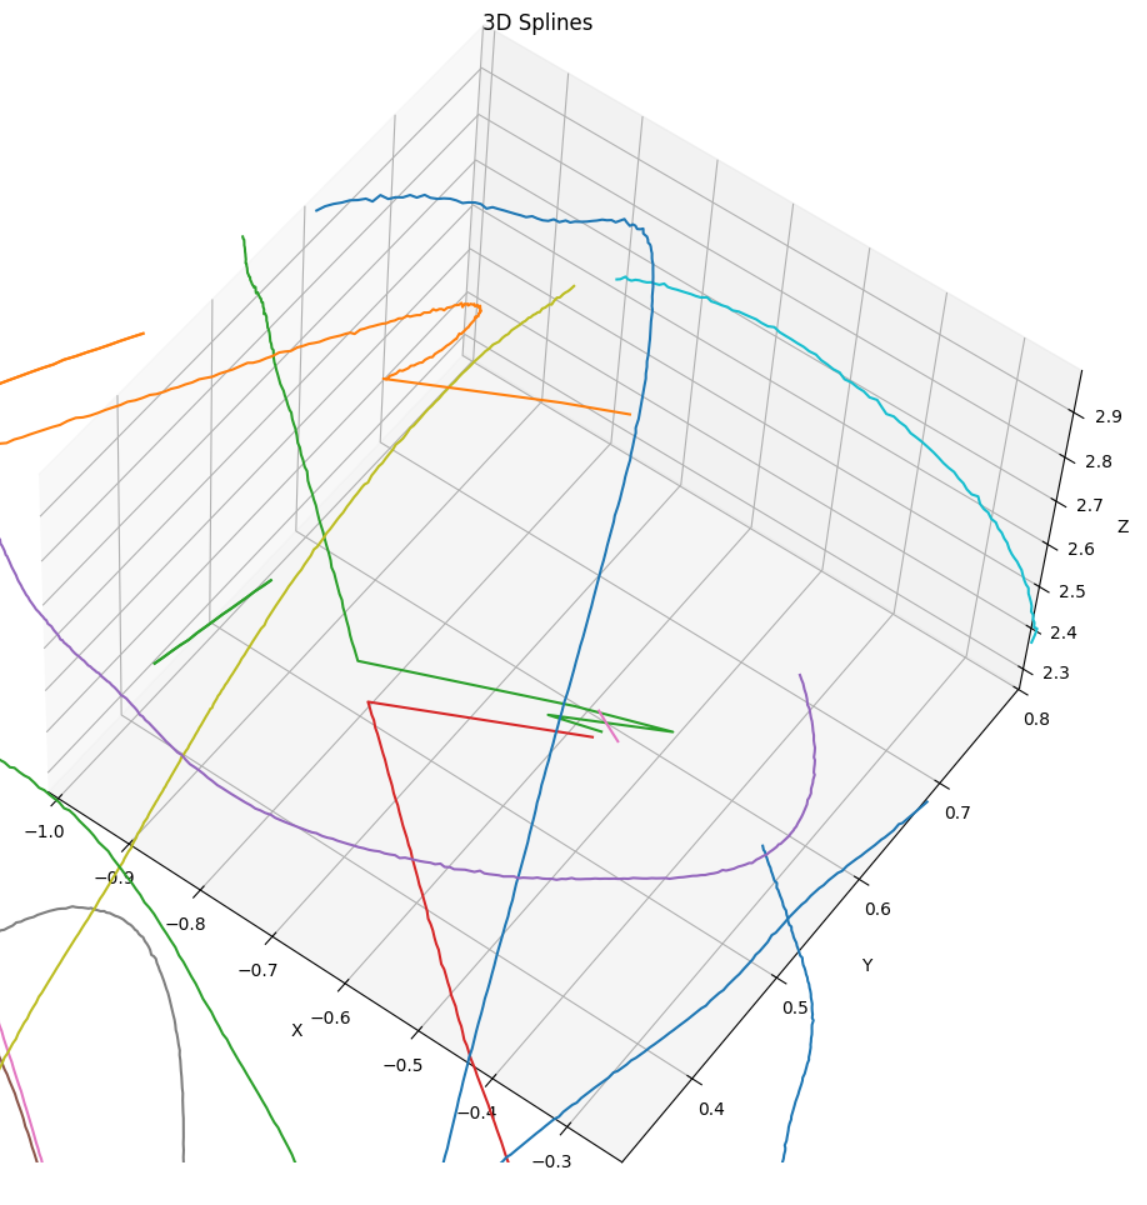
\includegraphics[width=0.6\textwidth]{imgs/splines_discontinuity.png}
    \caption{Example of the discontinuity in the 3D splines (dataset 4)}
    \label{fig:splines_discontinuity}
\end{figure}

This problem triggered a cascade effect: the inaccuracies in the 3D splines led to poor triangulation of new points, which in turn caused further inaccuracies in the camera poses.

In particular, for the reasons above we weren't able to reconstruct the 3D trajectory at all with the offline approach for the dataset3

\subsection{Online Trajectory Reconstruction}

The online trajectory reconstruction algorithm suffered from similar limitations as the offline one, and they were even more pronounced due to the real-time nature of the implementation.

Since the dataset provided ground truth for $\alpha,\beta$ parameters only for datasets 3 and 4, we could test the online trajectory reconstruction only on these datasets.

The lower number of correspondences available for each camera pair made the computed \textit{F} less reliable, and the algorithm was more prone to accumulating errors. This led to a more pronounced drift in the 3D trajectory (Figure \ref{fig:online_noisy_detections}), which was not corrected by the bundle adjustment step.

\begin{figure}[h]
    \centering
    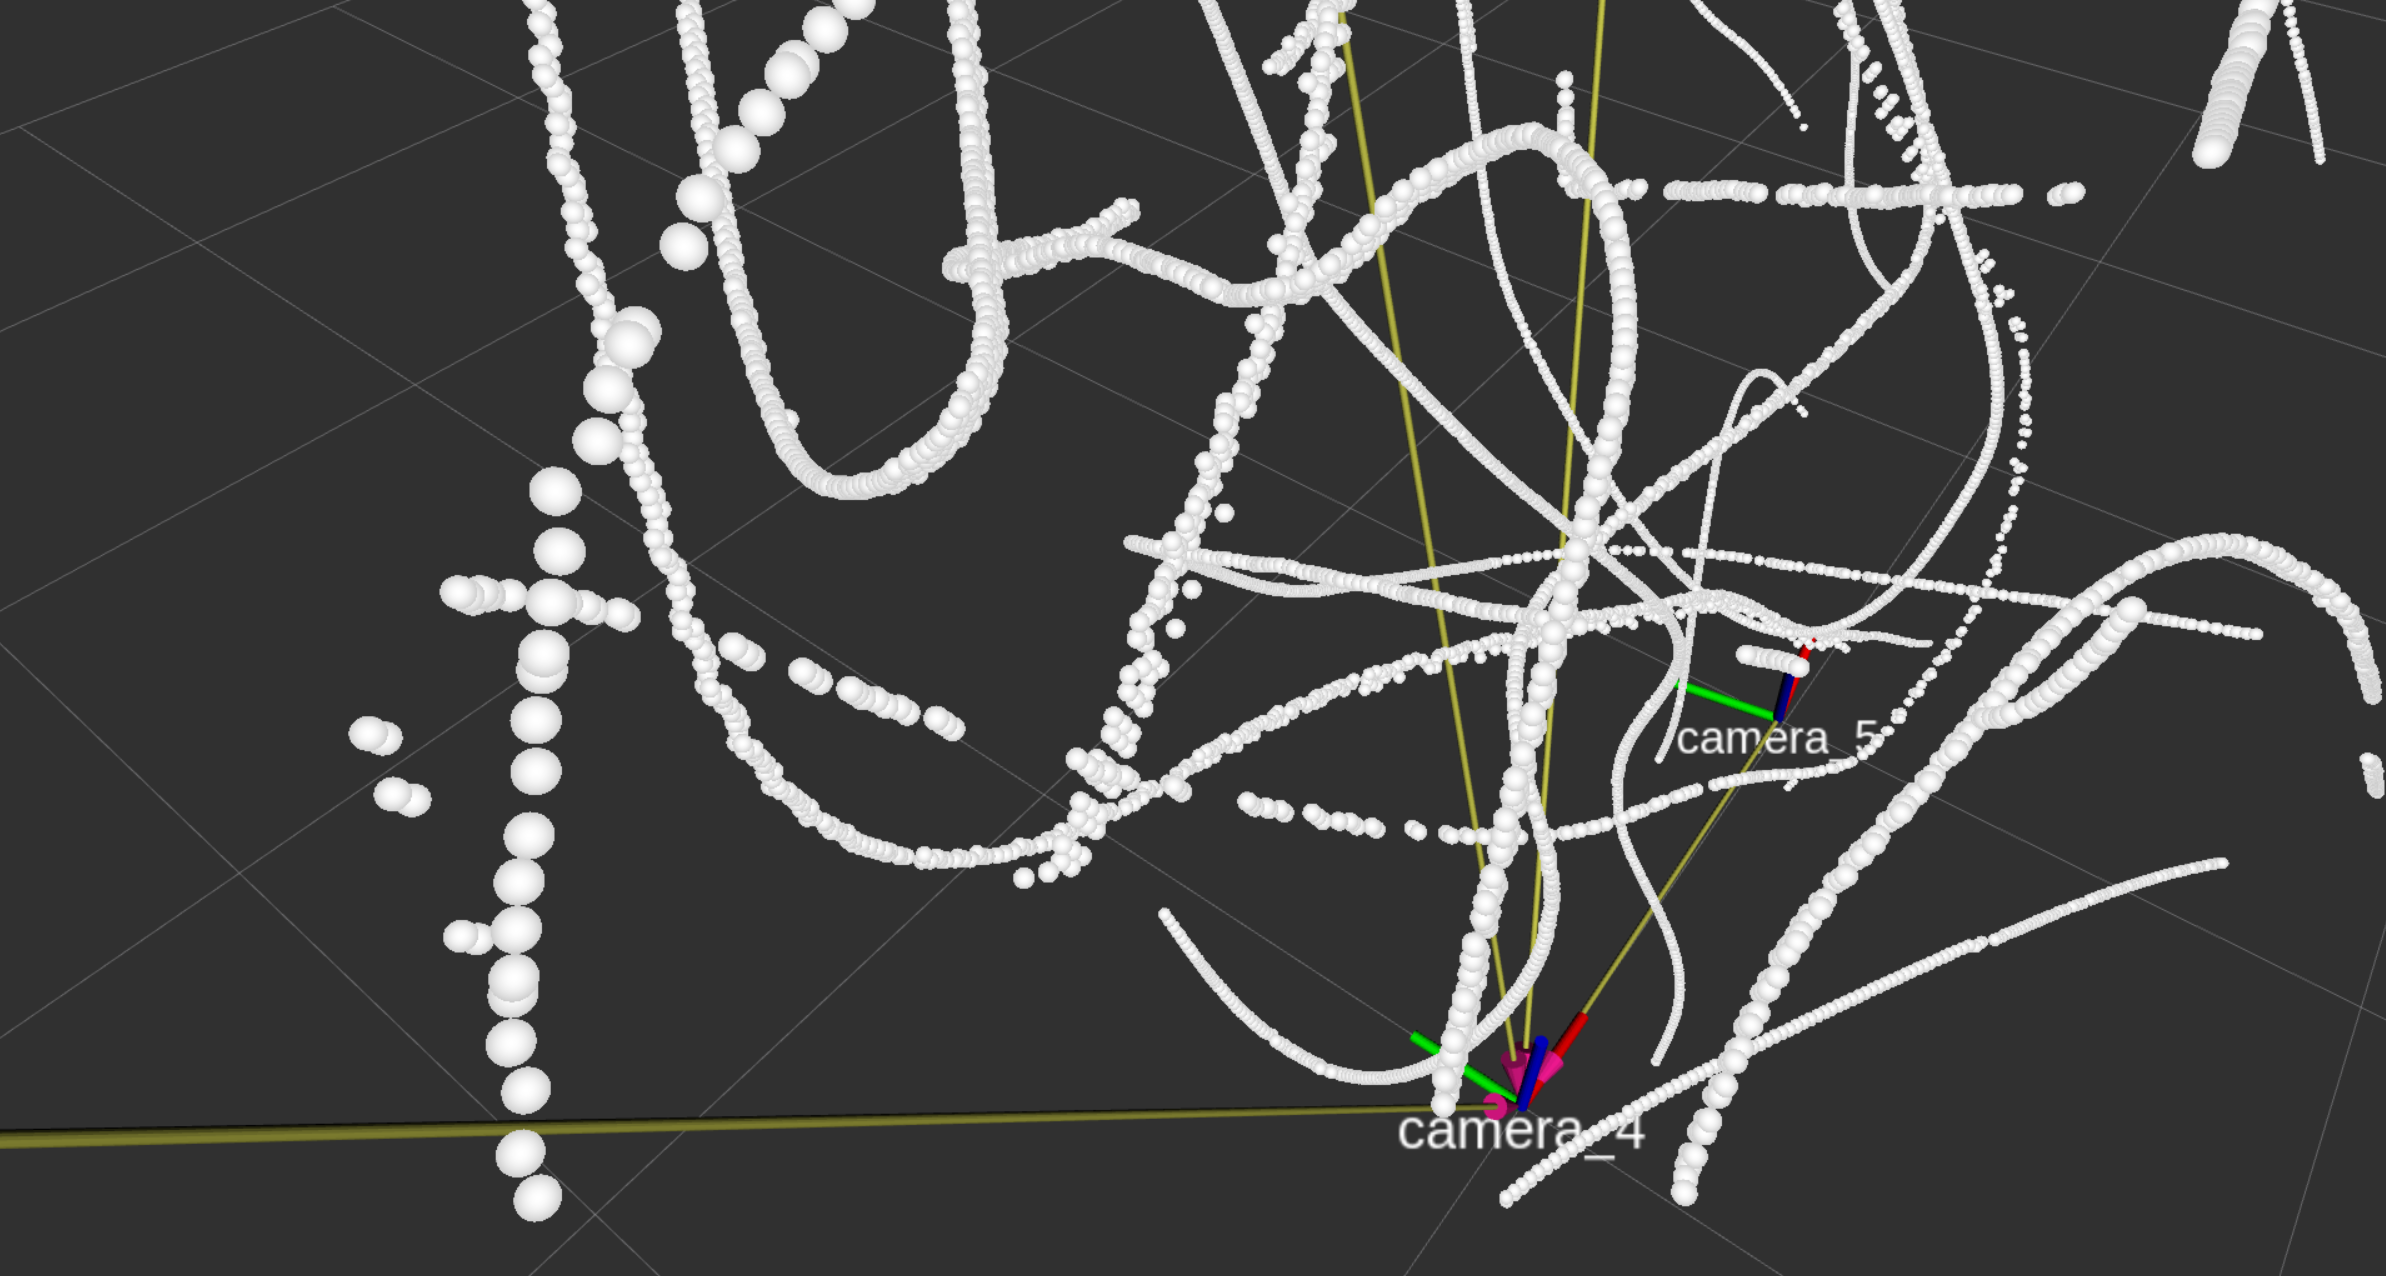
\includegraphics[width=0.5\textwidth]{imgs/online_noisy_detections.png}
    \caption{Example of the noisy drone detections in the online trajectory reconstruction (dataset 4)}
    \label{fig:online_noisy_detections}
\end{figure}

The 3D splines were so noisy that the bundle adjustment step actually worsened the results, introducing more errors instead of correcting them. This effect is illustrated in Figure \ref{fig:bad_ba_online}. This cycle of errors often led to the inability to produce a trajectory at all (Figure \ref{fig:bad_ba_online_failed}).

\begin{figure}[h]
    \centering
    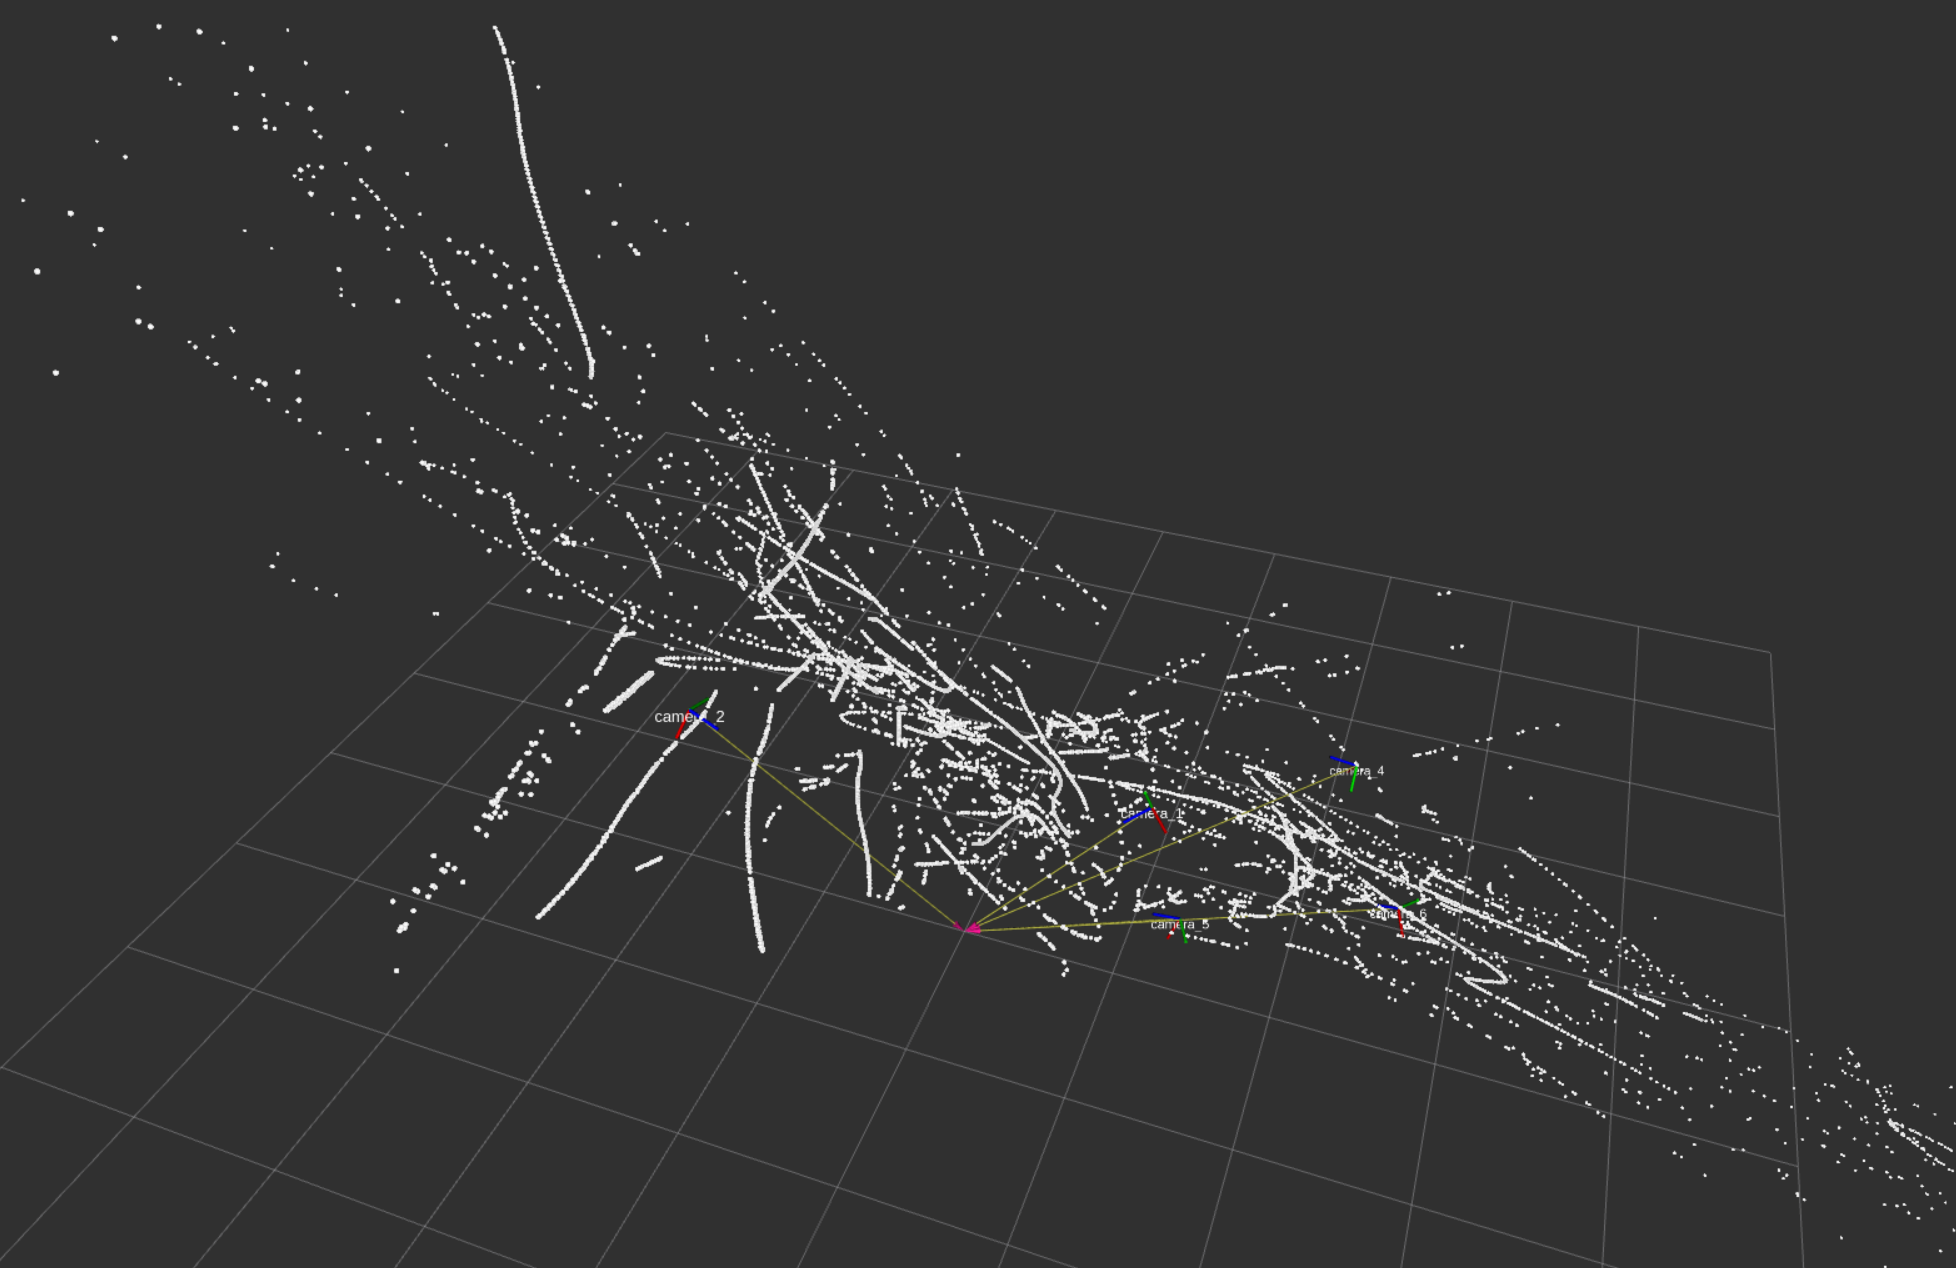
\includegraphics[width=0.5\textwidth]{imgs/online_failed_due_to_ba.png}
    \caption{Example of the algorithm failing to produce a trajectory due to bundle adjustment introducing too many errors.}
    \label{fig:bad_ba_online_failed}
\end{figure}

A new issue was also introduced by the real-time nature of the implementation: the algorithm was not able to correctly handle the fisheye camera (gopro3); we think that this was due to the fact that the fisheye camera was calibrated as a pinhole camera, and therefore the computation of its distortion coefficients in the intrinsic calibration step was not accurate enough. To mitigate this issue, we decided to ignore the fisheye camera in the online trajectory reconstruction, as it was not essential for the trajectory reconstruction. In future work, we could try to distinct between pinhole and fisheye cameras, and apply a different rectification method for each type of camera.\\

The dataset also provided the ground truth trajectory for the drone in some case. Unfortunately, due to the limitations above mentioned for both methods, the reconstructed trajectory was not accurate enough to be compared with the ground truth, so we had to skip the comparison step. However, we can still qualitatively assess the performance of the algorithm by visualizing the reconstructed trajectory in 3D space, as shown in Figures \ref{fig:online_full_trajectory}, \ref{fig:3d_splines_extension}.

\section{Instructions to run the code}

Since we implemented both the offline and online trajectory reconstruction algorithms, we provided two different scripts to run them.

\subsection{Environment setup}

Since the project relies on the dataset provided by the authors of the paper that is publicly available on GitHub (and, moreover, quite large), we decided to not include it in the repository. We directly cloned the dataset repository in the root directory of our project, and made some little modifications:

\begin{itemize}
    \item We extracted each video from the original dataset and saved each video in the same folder as their compressed version
    \item Some cameras in the dataset are provided with two versions of calibration files (e.g. mate10): for a easier automatic loading of the calibration files, we kept only one of the two versions, removing the suffix \texttt{\_1} or \texttt{\_2} from the file name. This way, the code can load the calibration files without having to specify which version to use.
\end{itemize}

Said that, in order to run the code, you need to have all the Python dependencies installed, this can be done by running the following command in the root directory of the project:

\begin{verbatim}
pip install -r requirements.txt
\end{verbatim}

\subsection{Camera Intrinsic Calibration}

The camera intrinsic calibration can be run by executing the following command:

\begin{verbatim}
python camera_calib.py
\end{verbatim}

This script will automatically load the checkerboard images from the dataset, detect the corners, compute the intrinsic parameters, and save both the intrinsic parameters (in a \texttt{json} file) and the plots showing the comparison between the computed intrinsic parameters and the ground truth values provided in the dataset. The plots will be saved in the \texttt{plots/intrinsic\_calibration/} folder.

\subsection{Drone Detection}

The drone detection algorithm can be run by executing a single Python script, with appropriate arguments:

\begin{verbatim}
python moving_video.py [-h] [--y_limit Y_LIMIT] dataset camera

Drone tracking with background subtraction and optical flow.

positional arguments:
  dataset            Dataset number
  camera             Camera number

options:
  --y_limit Y_LIMIT  Y limit for search area (default: 1080)
\end{verbatim}

This script will save in the \texttt{plots/} folder a \texttt{mp4} video with the drone detections overlaid on the original video (image \ref{fig:drone_detection} is a frame of this video), a \texttt{json} file with the drone detections, and an image with the analysis of the results of the background subtraction algorithm (image \ref{fig:detection_plots}), and the same set of files for the optical flow algorithm.

\subsection{Offline Trajectory Reconstruction}

The offline trajectory reconstruction is divided in two scripts, one for the $\beta$ search and one for the trajectory reconstruction. We decided to split the two scripts since the first one is quite time consuming, and it can be run only once for each dataset.

To run the $\beta$ search, you can execute the following command:

\begin{verbatim}
python beta_search.py dataset_no
\end{verbatim}

Where \texttt{dataset\_no} is the number of the dataset you want to use. This script will save in the \texttt{plots/search\_results/} folder all the plots showing the results of the $\beta$ search, and in the main directory a \texttt{csv} file with the results of the search, named \texttt{beta\_results\_dataset\_X.csv}, where \texttt{X} is the dataset number.

To run the trajectory reconstruction, you can execute the following command:

\begin{verbatim}
python main.py [-h] dataset_no

3D Spline Reconstruction

positional arguments:
  dataset_no  Dataset number to use
\end{verbatim}

This script will execute all the steps described in above, saving all the results in the \texttt{plots/} folder. To see the results, in a more interactive way, you can uncomment the very last line of the script, which will display all the intermediate results (Note: this will open a lot of windows, so it is recommended to comment it back after you are done).

Even if it is heavily parallelized, the $\beta$ search is still very time consuming. For this reason, we suggest not to delete the \texttt{csv} files named \texttt{beta\_results\_dataset\_X.csv}, since the trajectory reconstruction script will automatically load the results from these files, and it will fail if they are not present.

\subsection{Online Trajectory Reconstruction}

The online trajectory reconstruction is a bit more complex, as it requires ROS2 to be installed and running.

The code is structured in a ROS2 package, that has to be put in the \texttt{src/} folder of a ROS2 workspace. For semplicity, we already attached the ROS2 bag file containing the live drone detections, so you can run the online trajectory reconstruction without having to generate the bag file yourself. However, if you want to generate the bag, you can follow the instructions below.

The bag generation can be done by putting the \texttt{csv} file with the drone detections generated in the offline trajectory reconstruction step in the same location from which you want to run the ROS2 node, and then running the following command:

\begin{verbatim}
    colcon build
    source install/setup.bash
    ros2 run drones live_detections_generator
\end{verbatim}

This will publish the drone detections in a ROS2 topic, and in order to save them in a ROS2 bag file, you can run the following command in another terminal:

\begin{verbatim}
    ros2 bag record -o <name_of_the_bag_file> /detections
\end{verbatim}

To run the online trajectory reconstruction, you need to follow these steps (assuming you are in the ROS2 workspace root directory):

\begin{verbatim}
    colcon build
    source install/setup.bash
    ros2 run drones drones
\end{verbatim}

It is important to select the correct dataset number in the \texttt{drones.py} file, as the code is hardcoded to use the dataset 3 or 4. The dataset number can be changed in the first lines of the \texttt{drones.py} file, where you can also change the parameters of the algorithm.

Then, in another terminal:

\begin{verbatim}
ros2 bag play <path_to_the_bag_file> -r <0.2 | 1.5>
\end{verbatim}

This will start the ROS2 node that reconstructs the drone trajectory in real-time, and it will replay the bag file containing the drone detections (the bag file is already provided in the repository). The rate of the replay can be adjusted with the \texttt{-r} option, but we suggest to keep it at 1.5x the original speed for dataset 4 and 0.2 for dataset 3, as this is the speed that most closely resembles the real-time time flow of the dataset.

To keep the node implementation as simple as possible, instead of following the ROS2 conventions and having a launch file and a configuration file, we decided to hardcode the parameters in the node itself. This means that you will have to modify the first lines of the \texttt{drones.py} file to change the parameters of the algorithm.

\section{Content of the repository}

The repository contains the following folders and files:
\begin{itemize}
    \item \texttt{plots/}: Contains all output results from each step of the project. This includes:
          \begin{itemize}
              \item Intrinsic calibration results for each camera, with comparisons to the dataset's ground truth.
              \item Drone detection results for all three methods (background subtraction, optical flow, YOLOv8), including overlaid videos, \texttt{json} files with detections, and analysis plots (provided for a subset of videos to keep the repository size manageable).
              \item Offline trajectory reconstruction results, organized by dataset.
              \item Online trajectory reconstruction results, including videos showing live trajectory construction.
              \item Results of the $\beta$ search for temporal alignment.
          \end{itemize}
    \item \texttt{ros\_node/}: Contains the ROS2 package for online trajectory reconstruction, structured as follows:
          \begin{itemize}
              \item \texttt{bags/}: ROS2 bag files for datasets 3 and 4, used to test the online trajectory reconstruction.
              \item \texttt{config/rviz2\_config.yaml.rviz2}: RViz2 configuration file for visualizing the reconstructed trajectory and camera positions.
              \item \texttt{drones/drones.py}: Main ROS2 node that performs real-time drone trajectory reconstruction.
              \item \texttt{drones/live\_detections\_generator.py}: ROS2 node that publishes live drone detections from the \texttt{csv} files.
          \end{itemize}
    \item Other files: These include the CSV files listing the $\beta$ values found for each dataset, as well as the main scripts for running the offline trajectory reconstruction and drone detection algorithms.
\end{itemize}

All the scripts are well commented, so they should be easy to understand and modify.


\section{Conclusions}

This project presents a robust and modular implementation of a drone trajectory reconstruction pipeline, inspired by state-of-the-art methods in outside-in tracking with unsynchronized cameras. The implementation covers key components, with careful integration of computer vision tools and frameworks like OpenCV and ROS2. Although the pipeline suffers from several limitations, it demonstrates strong potential for scalable, low-cost UAV tracking in real-world conditions.

Future improvements could focus on refining the bundle adjustment process to incorporate motion regularization, improving robustness to camera variability, and enhancing the detection component for better performance in occluded or low-visibility scenarios. Despite the challenges, this work serves as a strong foundation for further research and development in drone tracking systems using consumer-grade equipment.

\section*{Bulky Plots}

In order to keep the report clean and readable, we decided to move the bulkiest plots to the end of the document

\begin{figure}[h]
    \centering
    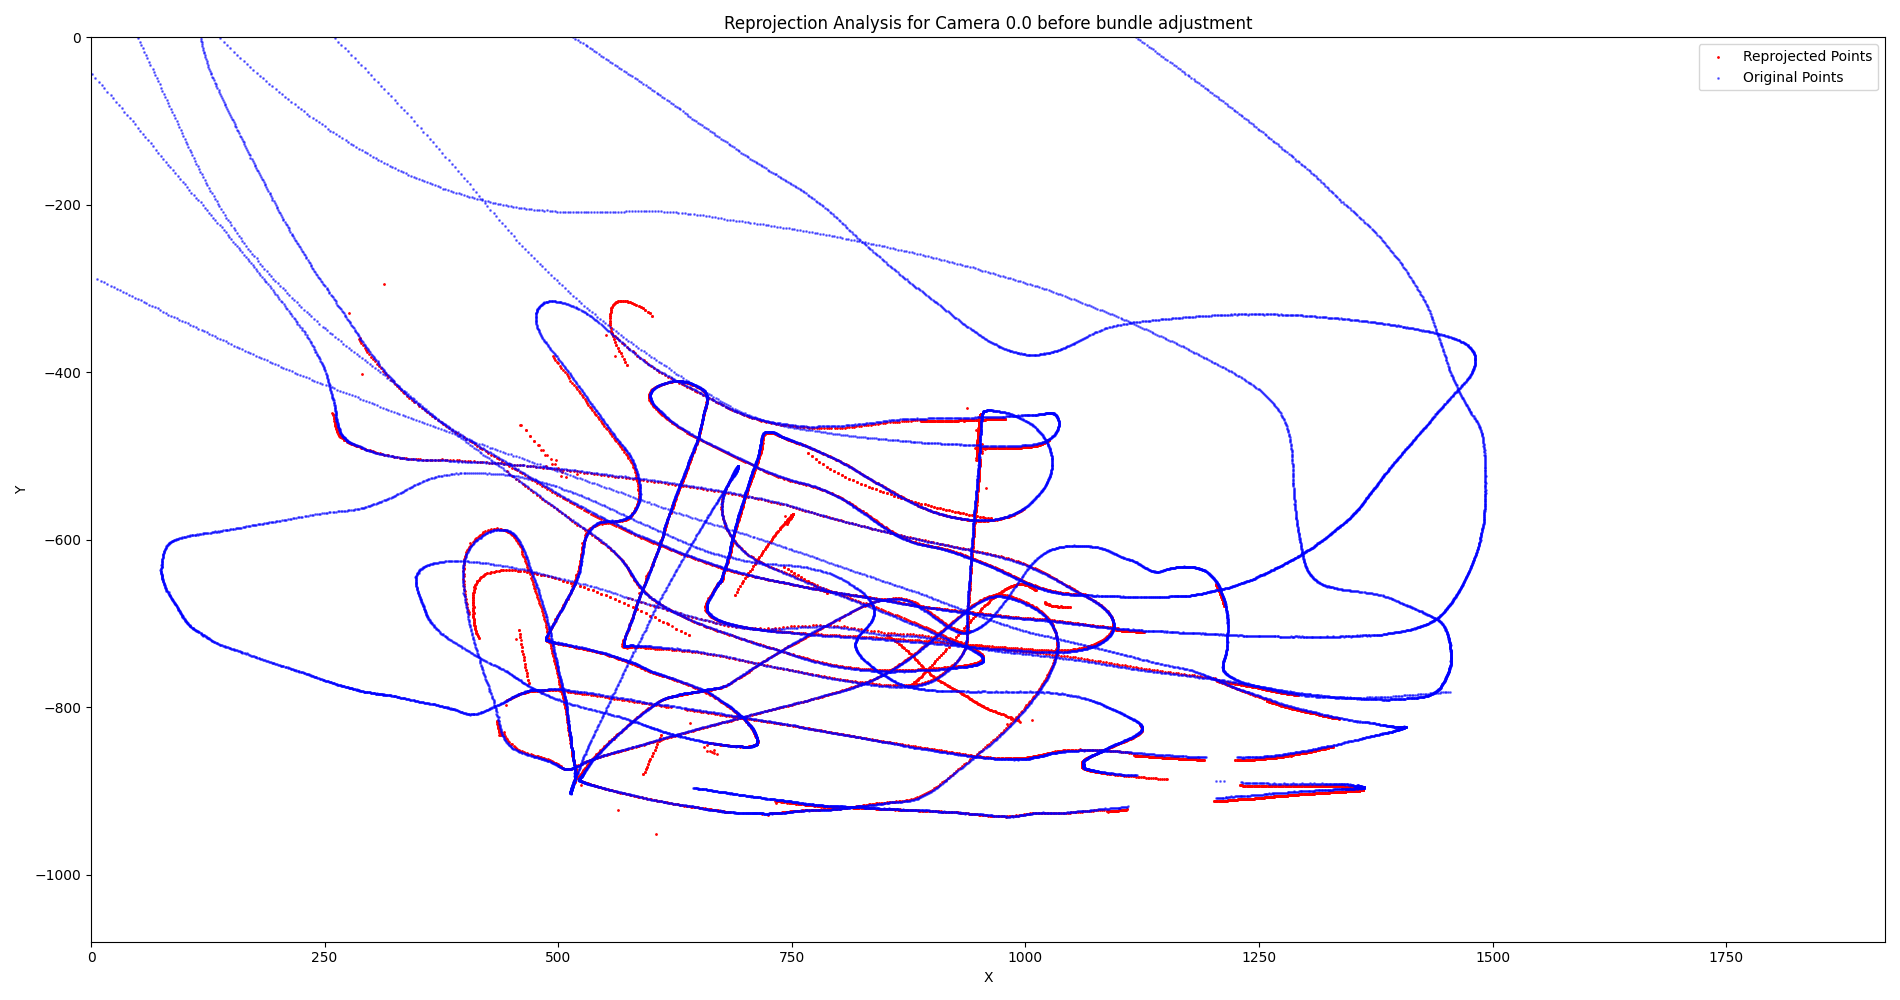
\includegraphics[width=\textwidth]{../plots/dataset4/reprojection_analysis_camera_0_before_ba_.png}
    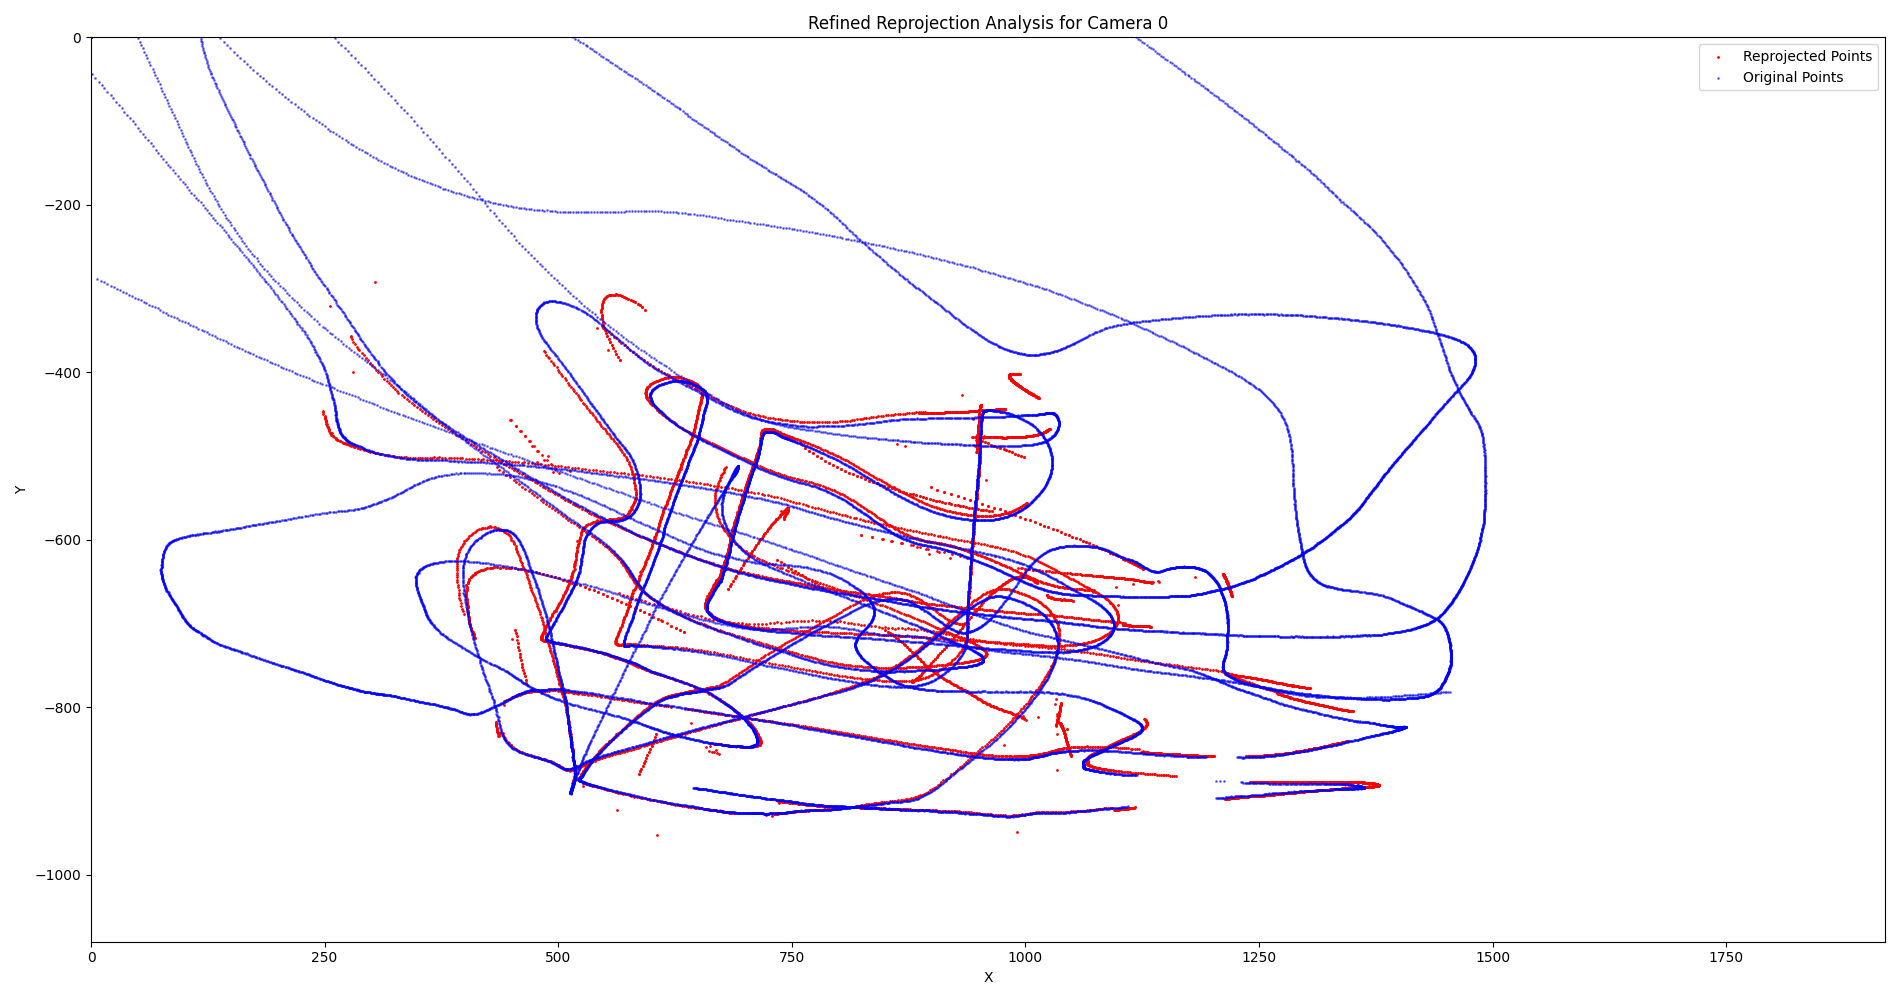
\includegraphics[width=\textwidth]{../plots/dataset4/reprojection_analysis_camera_0.png}
    \caption{Offline approach - Reprojection error analysis for camera 0 (dataset 4). The top plot shows the reprojection error before the bundle adjustment, while the bottom plot shows the reprojection error after the bundle adjustment}
    \label{fig:reprojection_analysis}
\end{figure}

\begin{figure}[h]
    \centering
    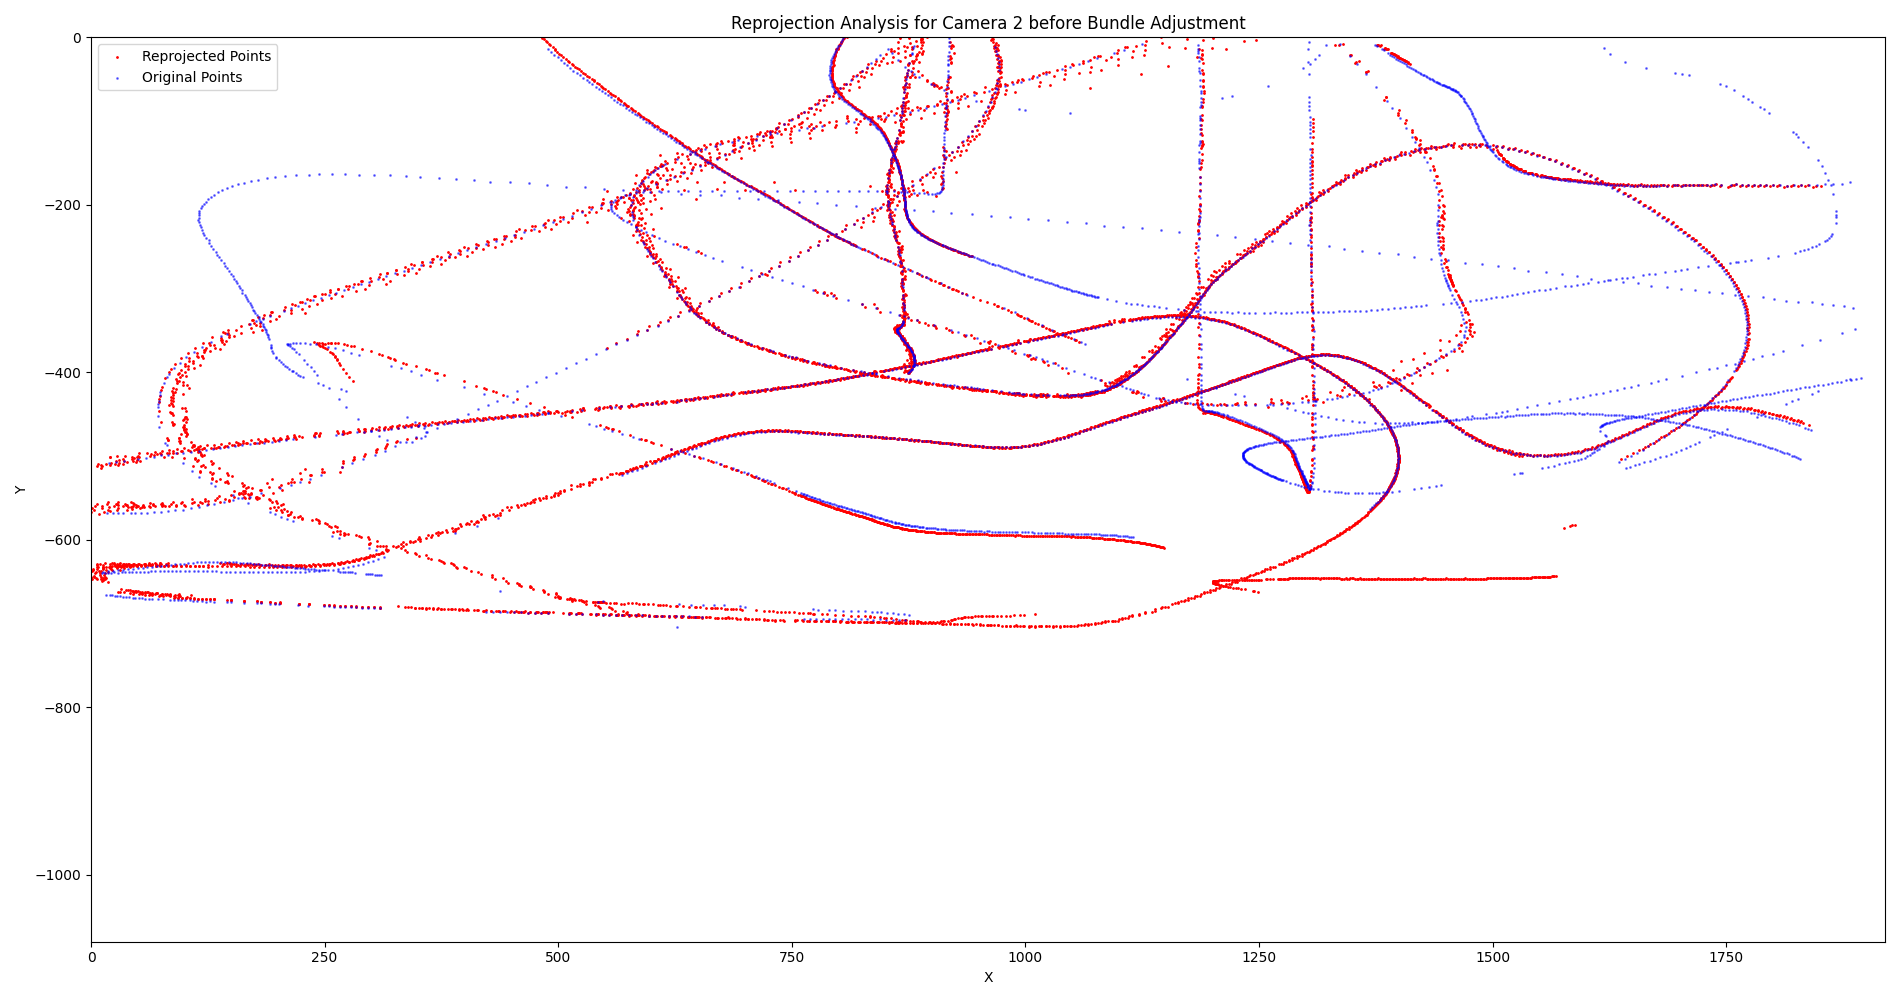
\includegraphics[width=\textwidth]{imgs/online_no_ba_cam2.png}
    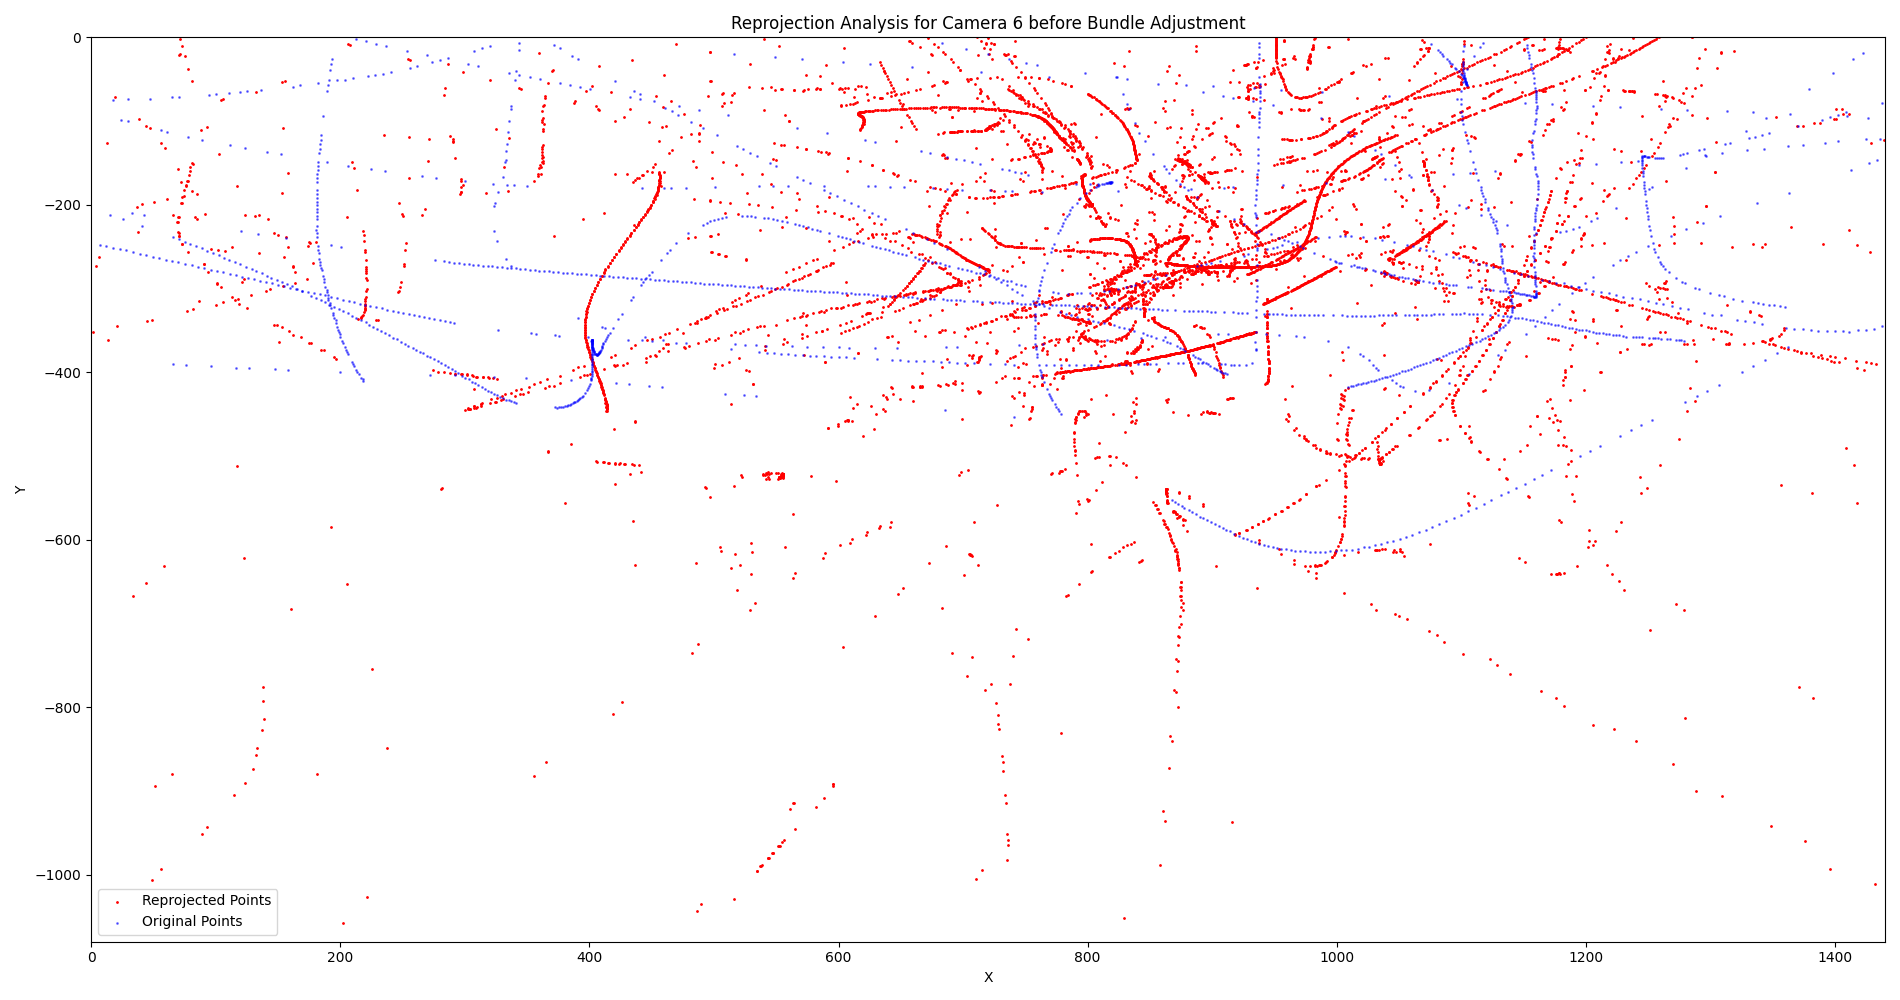
\includegraphics[width=\textwidth]{imgs/online_ba_cam2.png}
    \caption{Online approach - Reprojection error for camera 2 (dataset 4): before (top) and after (bottom) bundle adjustment. The bundle adjustment worsens the results, most likely due to the noisy (although plausible) 3D splines}
    \label{fig:bad_ba_online}
\end{figure}

\begin{figure}[h]
    \centering
    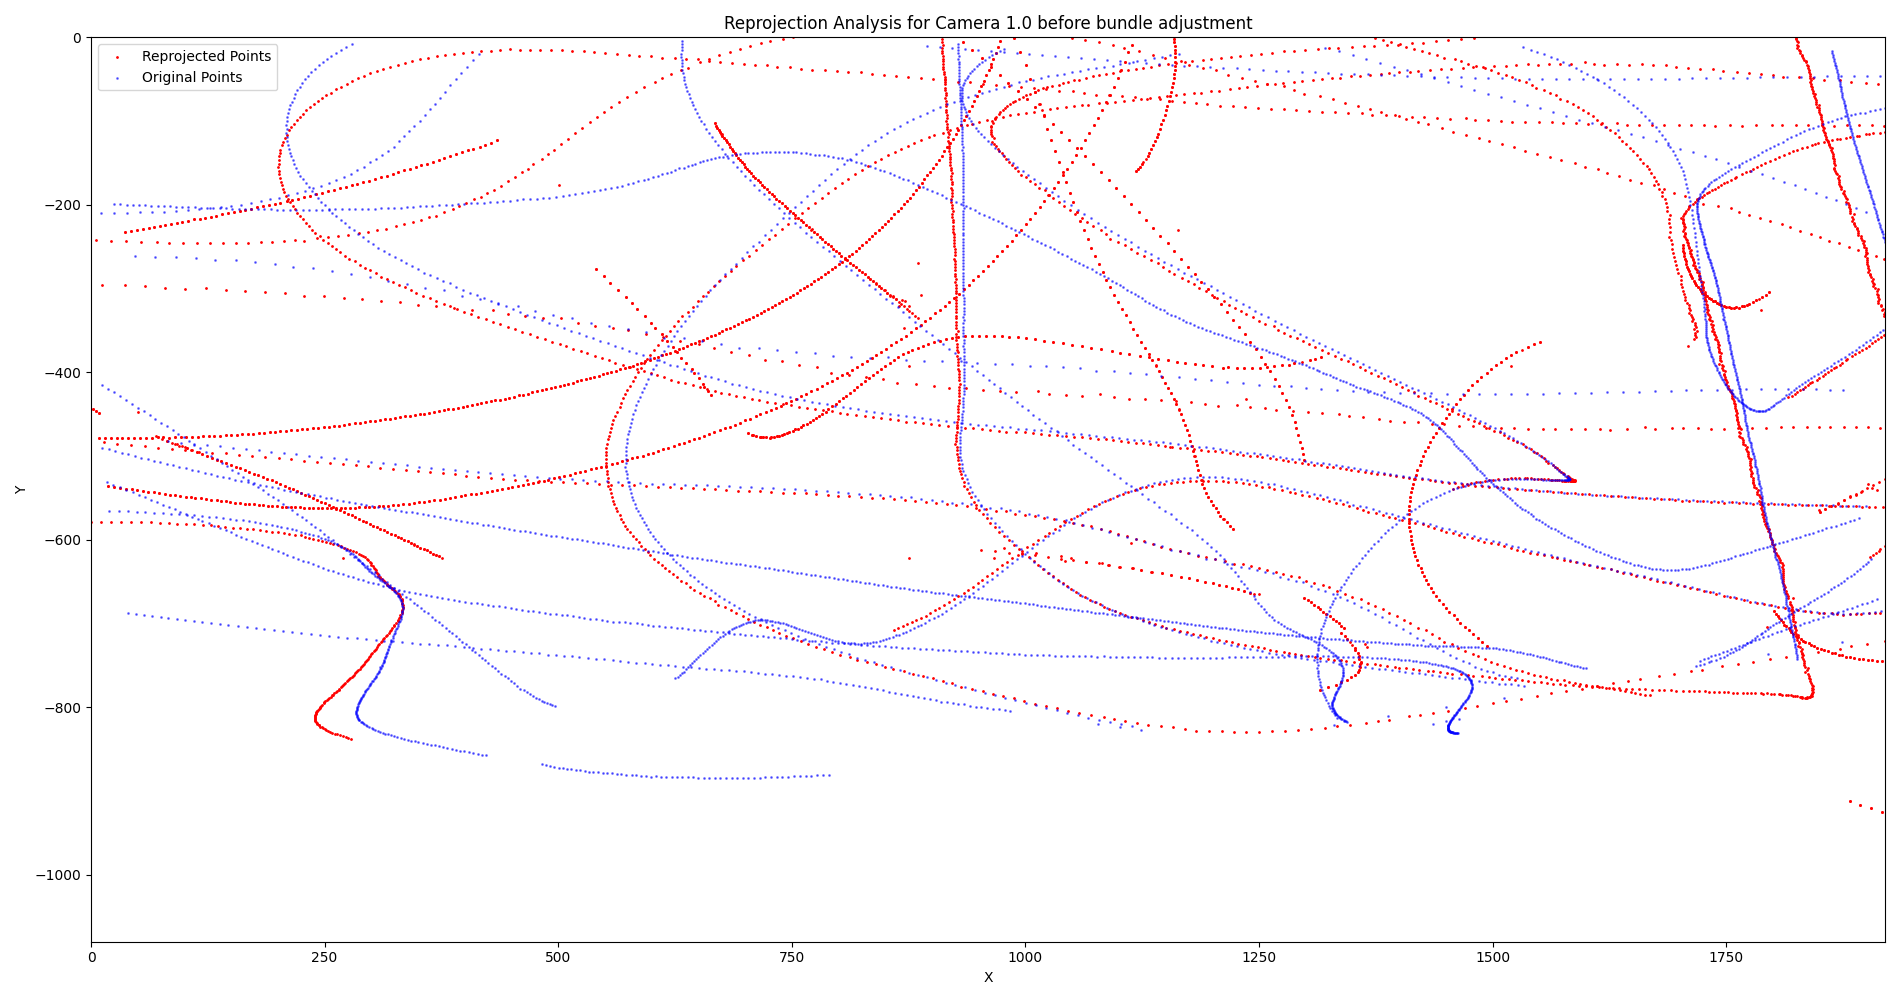
\includegraphics[width=\textwidth]{../plots/dataset4/reprojection_analysis_camera_1_before_ba_.png}
    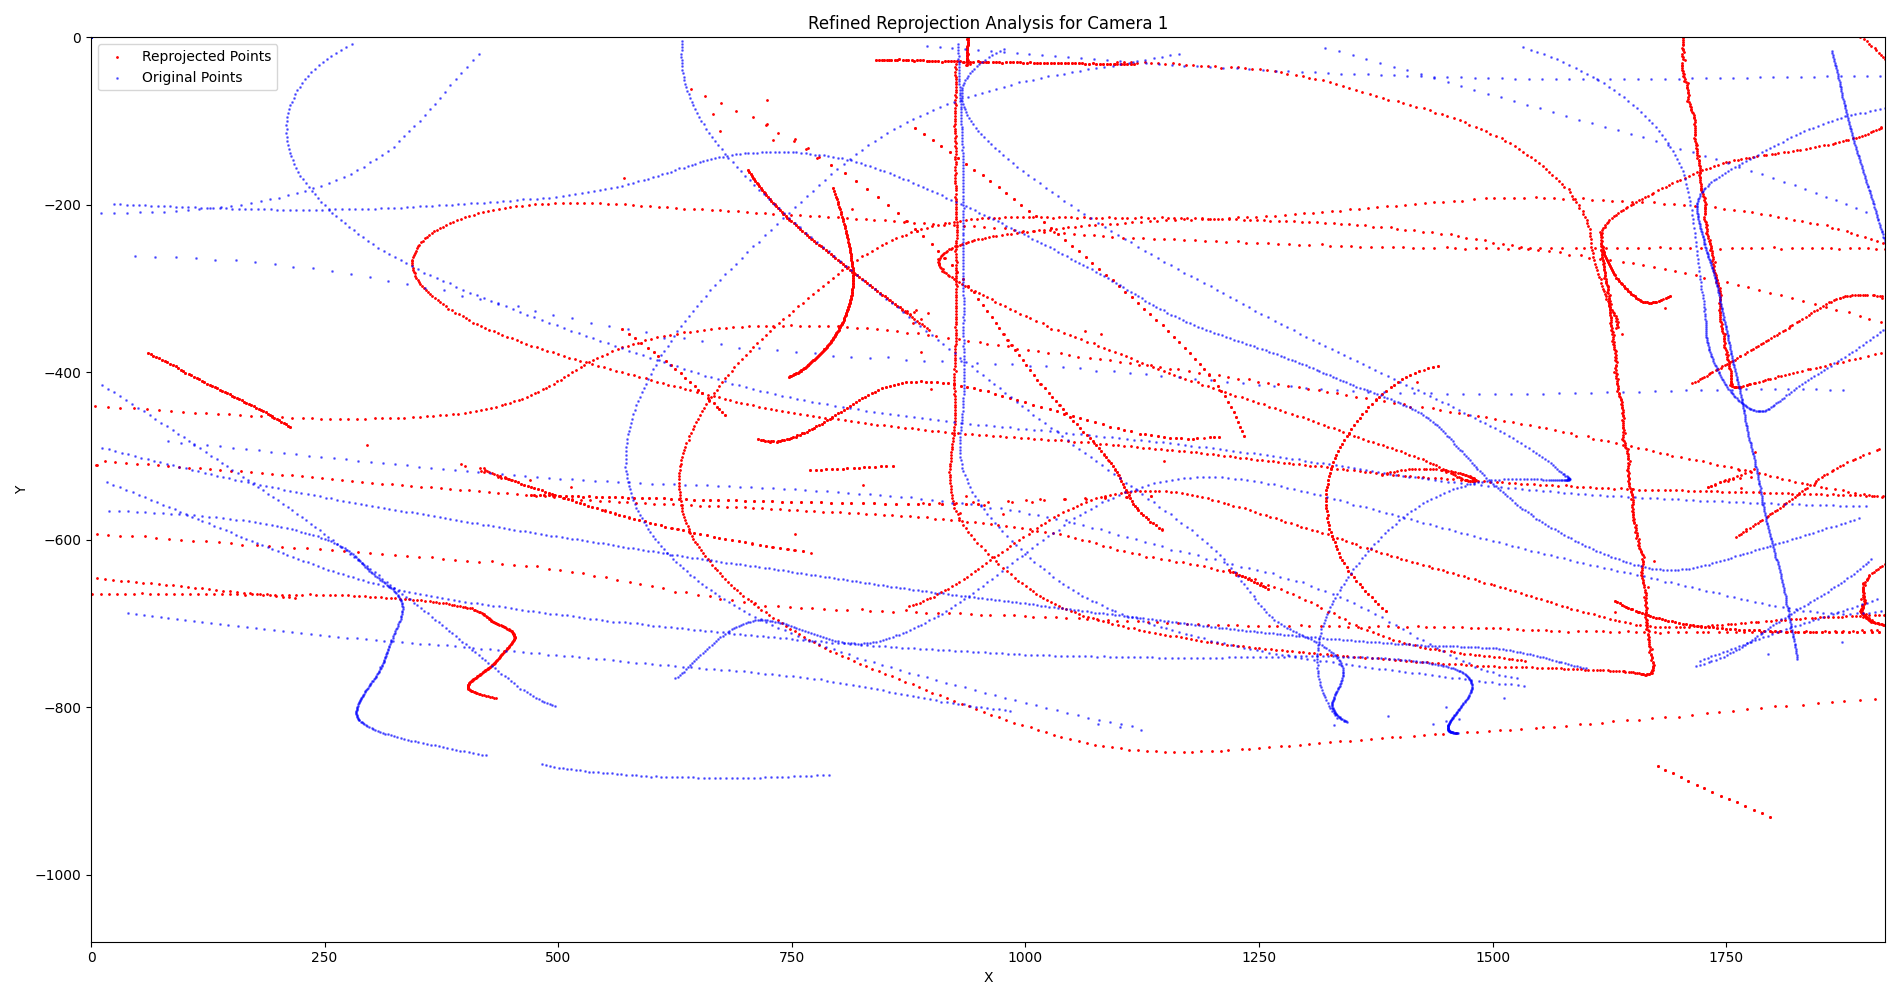
\includegraphics[width=\textwidth]{../plots/dataset4/reprojection_analysis_camera_1.png}
    \caption{Offline approach - Reprojection error analysis for camera 1 (dataset 4). The top plot shows the reprojection error before the bundle adjustment, while the bottom plot shows the reprojection error after the bundle adjustment. It is clear that the bundle adjustment completely fails to refine the trajectory, as the 3D splines are not consistent}
    \label{fig:bad_ba}
\end{figure}

\end{document}